Like all industrial processes, Powder Bed Fusion (PBF) relies on process parameters control to ensure proper functioning. When a process shows the expected behavior, it is called an "in-control process". On the other hand, when the process deviates from the desired behavior, its output becomes unpredictable and is referred to as "out-of-control" (OOC). When a process is out of control, anomalies and defects can arise in the output. Section \ref{sec:defects} describes the most common defects in PBF processes and their causes, while Section \ref{sec:comelotrovo} presents different approaches for defect detection. Section \ref{sec:sensoriniiniini} reports an overview of available sensors used in anomaly detection.  Sections of this chapter are mainly based on \citeauthor{grasso_-process_2017} (2017), \citeauthor{grasso_process_2017} (2017), \citeauthor{mostafaei_defects_2022} (2022) and \citeauthor{wu_additively_2023} (2023). Finally, Section \ref{sec:hotspot} focuses on defects caused by anomalies in the temperature profiles of the building bed.

% Categories of Defect in PBF Processes >>>
\section{Defects Categories in PBF Processes}
\label{sec:defects}
Defects in PBF processes can be divided into five main classes: porosity defects, residual stresses and cracking, geometric defects and dimensional accuracy, balling, and surface defects.
\paragraph{Porosity.} Porosity is a significant parameter for many metal AM applications, as it strongly impacts fatigue resistance and crack propagation in the component \cite{edwards_electron_2013}. 
\begin{figure}
    \centering
    \subfloat[\label{fig:poris}]{
        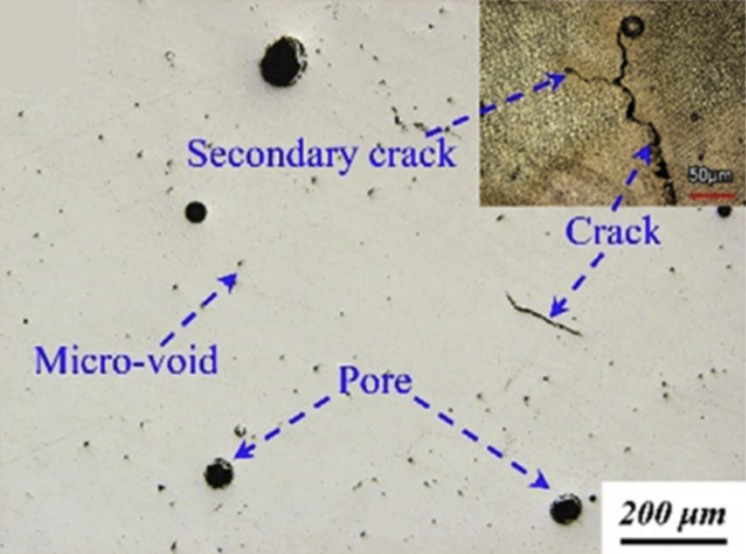
\includegraphics[scale=0.4]{Images/pori e crack.png}
    }
    \qquad
    \subfloat[\label{fig:acircular}]{
        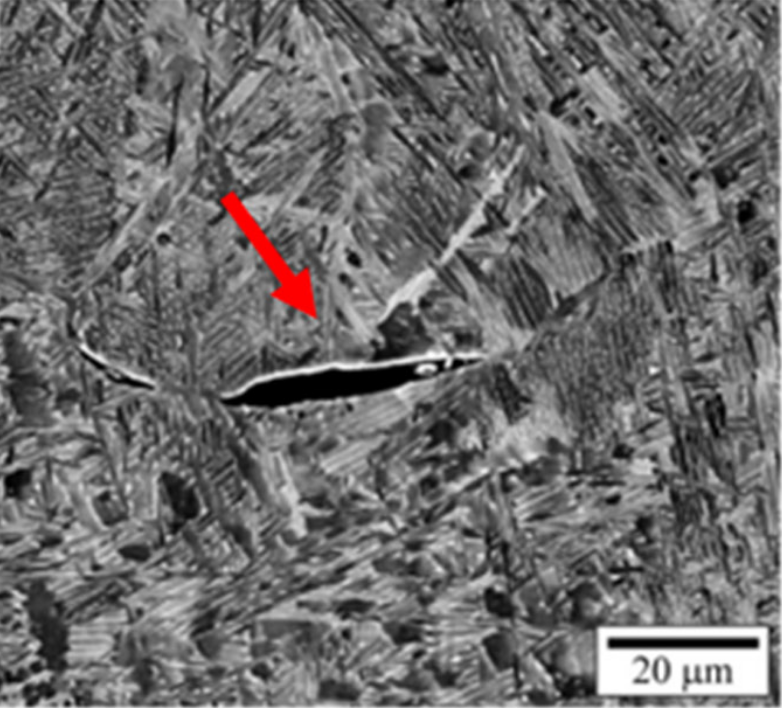
\includegraphics[scale=0.31]{Images/acircular.png}
    }
    \qquad
    \subfloat[\label{fig:delamination}]{
        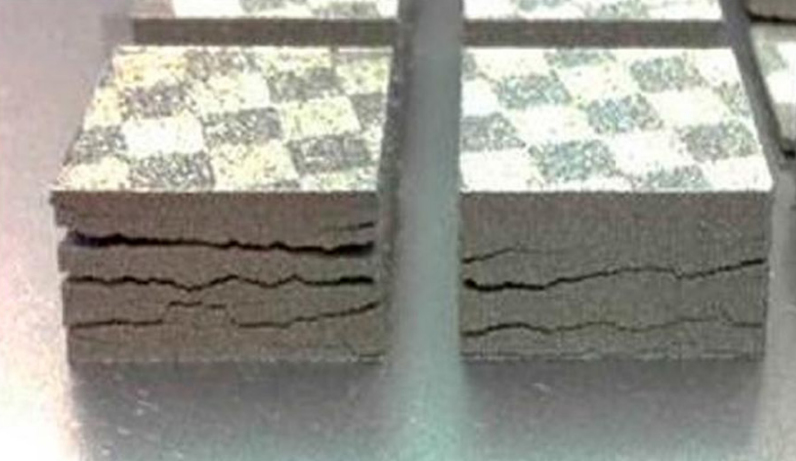
\includegraphics[scale=0.4]{Images/delamination.png}
    }
    \qquad
    \subfloat[\label{fig:balling}]{
        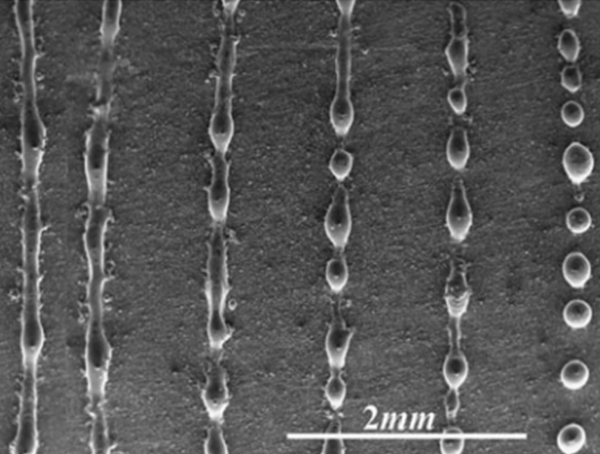
\includegraphics[scale=0.4]{Images/balling.png}
    }
    \caption[Defect examples in PBF.]{Pores, micro-void and cracks in a specimen of FeCrCoMnNi (a) \cite{mostafaei_defects_2022}, an acircular pores on a specimen of Ti–6Al–4V (b) \cite{tammas-williams_xct_2015}, an example of delamination in SLS (c) \cite{sames_metallurgy_2016} and the balling effect in stainless steal powder (d) \cite{li_balling_2012}.}
\end{figure} 
Porosity is characterized by empty spaces within the mass of the fused material. These voids can appear within a layer, between adjacent layers, or on the surface of the printed piece. Voids most frequently occur within the layer and can vary in size, form, and distribution. The primary causes for these pores include incomplete fusion in the powder bed (lack of fusion or LOF), keyhole effects, and encapsulated gas. We can also differentiate between round and non-round pores. Fig. \ref{fig:poris} shows some examples of round pores. The elongated voids observed between layers are called "acicular pores" and are characterized by a larger size. For example, the acircular pore in Fig. \ref{fig:acircular} has a measure of \SI{20}{\micro\metre}. Pores can be dispersed throughout the material or primarily situated below the surface, known as "under-skin pores". Pores can also appear on the exterior surface and are typically termed "surface porosities".
\paragraph{Residual stresses and delamination.} In material science, residual stresses are internal tensions that remain in the finished piece once the printing phase is complete. In PBF, these stresses can arise from two different causes: (i) the thermal gradient mechanism and (ii) the cool-down phase of molten top layers \cite{mercelis_residual_2006}. Cracking phenomena occur as a consequence of stress relief when the tensile stress exceeds the ultimate tensile strength of the solid material. When the tension is suddenly released, a secondary crack can be generated from the main crack. Fig. \ref{fig:poris} shows an example of this kind of defect. On the other hand, delamination happens when cracks originate and propagate between adjacent layers (inter-layer cracking). Delamination occurs when the residual stresses exceed the binding linkage between the top layer and the previous one. Most of the time, it happens from the partial disconnection of the part from the baseplate \cite{sames_metallurgy_2016}, as in Fig. \ref{fig:delamination}.
\begin{figure}
    \centering
    \subfloat[\label{fig:lackofsupport}]{
        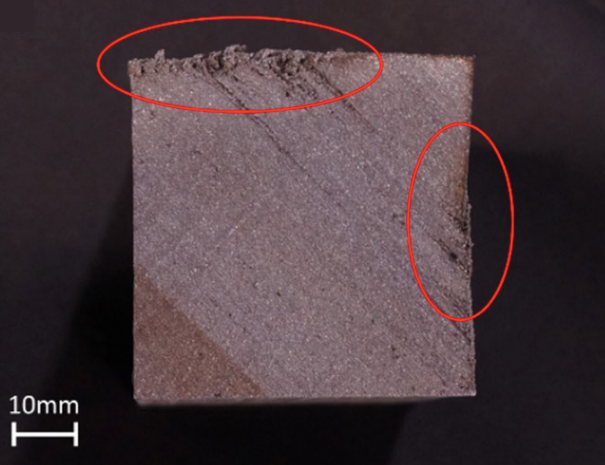
\includegraphics[scale=0.45]{Images/lackofsupport.png}
    }
    \qquad
    \subfloat[\label{fig:oxide}]{
        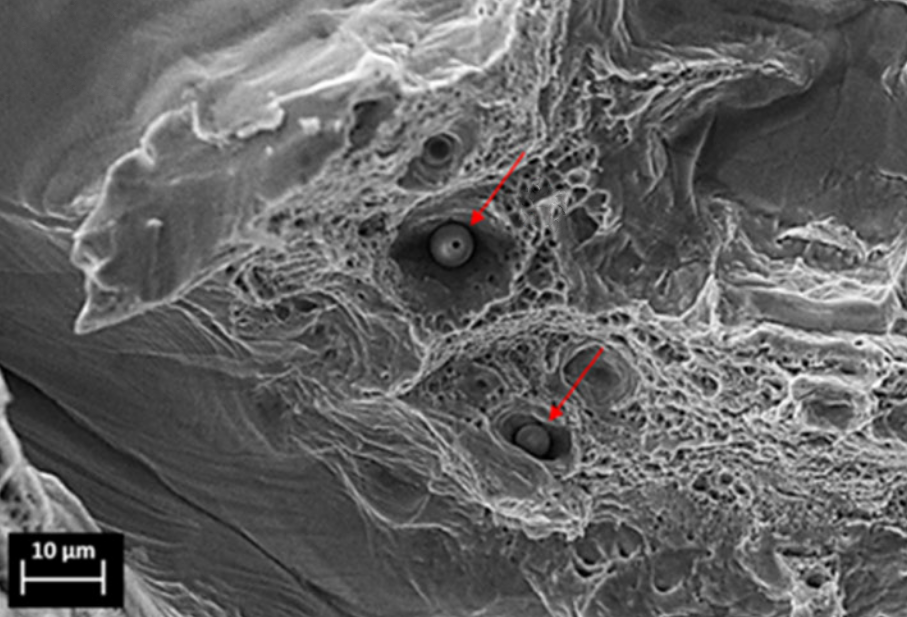
\includegraphics[scale=0.34]{Images/oxide.png}
    }
    \caption[Defects in PBF process.]{Example of geometrical errors in SLS caused by a wrong support (a) \cite{grasso_-process_2017} and examples of two local oxide contaminations (b) \cite{casati_microstructure_2016}.}
\end{figure} 
\paragraph{Geometric defects and dimensional accuracy.} Dimensional anomalies in PBF can be categorized into (i) contraction and expansion effects, (ii) warping and curling, (iii) dross formation on bottom-facing surfaces, (iv) super-elevated edges, and (v) additional on-plane geometric distortions. Contraction is among the more common defects, though the opposite effect (i.e., components that are consistently bigger than expected) might arise in specific scenarios. Warping occurs from heat dispersion processes and thermal tensions. Similarly, curling is a specific bending effect caused by inconsistent thermal growth and component shrinkage, generally tied to disparate contraction rates between the top and underside of overhanging segments. A combination of shrinking and warping effects results in curved outlines for bottom-facing surfaces intended to be flat. Super-elevated edges represent another type of OOC geometrical distortion, featuring elevated ridges of solidified material. Elevated edges not only compromise the final component's integrity but might also cause defect propagation since they can interfere with the recoating blade. Other distortions affect critical features such as thin walls, overhang areas, and acute corners. In correspondence with these features, the melt pool is surrounded mainly by loose powder, which has a lower conductivity than the solid material. The diminished heat flux yields local overheating phenomena that may deteriorate the geometric accuracy. This overheated area is called a hot spot (HS), and we will discuss it in Section \ref{sec:hotspot}.
\paragraph{Balling.} Melt ball formation, also called balling, occurs when the molten material solidifies into spheres instead of solid layers. This phenomenon is caused by surface tension, which prevents the molten material from spreading over the previous layer. The result is a rough and bead-shaped surface that produces an irregular layer deposition with detrimental effects on the density and quality of the final product. \citeauthor{li_balling_2012}(2012) pointed out three main problems when balling happens: (i) increased surface roughness, (ii) a large number of pores between the discontinuous metallic balls, and (iii) protruding spheres may interfere with the recoating blade. The latter happens only in the presence of a very severe balling effect. Fig. \ref{fig:balling} shows the balling effect on a stainless steel powder.
\paragraph{Surface defects.} In PBF methodologies, as in most AM processes, the texture of the surface is influenced by the layer-by-layer manufacturing process and by the existence of surface impurities, inconsistencies, and voids.
\begin{figure}
    \centering
    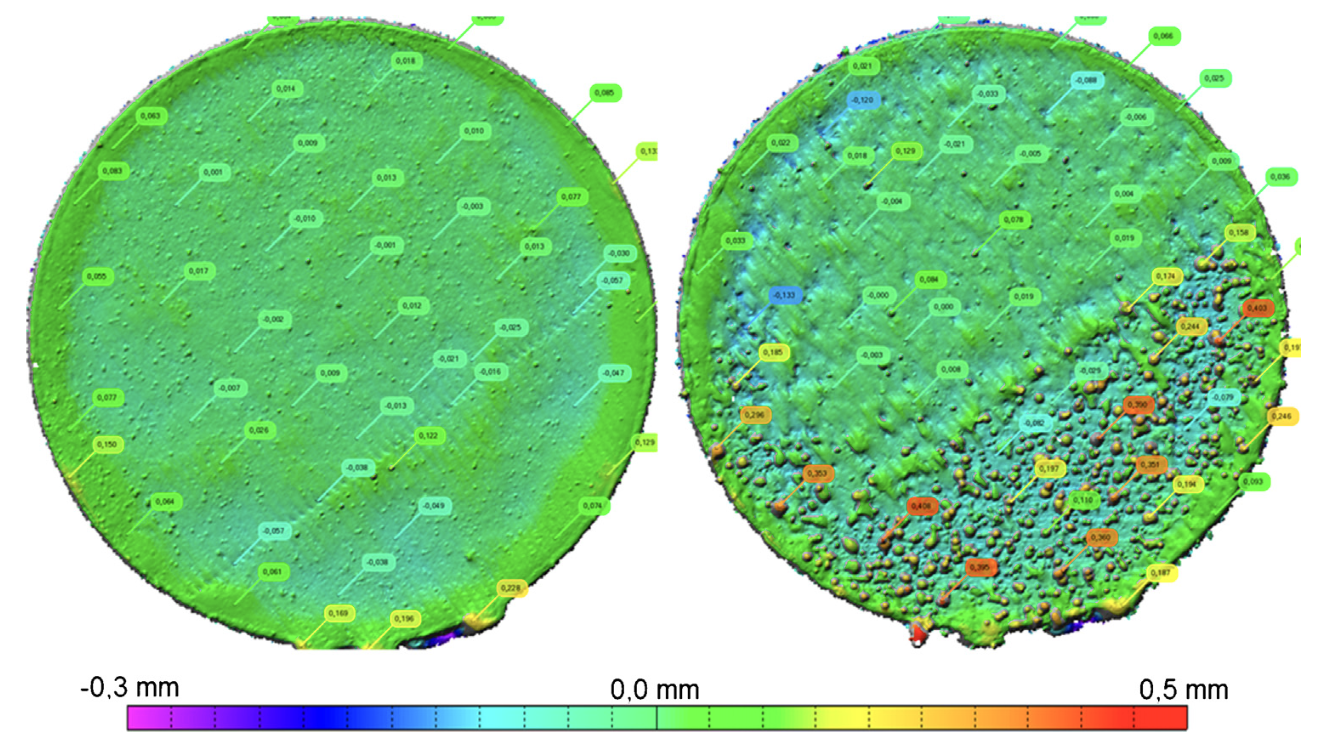
\includegraphics[scale=0.4]{Images/surface.png}
    \caption[Surface roughness in PBF]{Good (left) and poor (right) surface textures measured via confocal microscopy on parts produced either in the presence of good and improper gas flow conditions in L-PBF \cite{ladewig_influence_2016}.}
    \label{fig:surface}
\end{figure}
Processing conditions determine the surface's texture, the perimeter scanning technique, and the dimensions of powder particles. The orientation of the surface in relation to building direction influences its texture. In particular, downward-facing and upward-facing surfaces are known to have considerably different texture properties. Even though many parts produced via PBF are refined by post-processing operations (like surface polish and thermal procedures), the texture of the surface is of functional importance since it impacts the part's fatigue resilience. Furthermore, for medical lattice structures, the texture of the surface can help the implant's assimilation during bone healing. Fig. \ref{fig:surface} displays instances of optimal (left) and poor (right) surface textures as observed through confocal microscopy on components made under optimal and improper gas flow situations in L-PBF \cite{ladewig_influence_2016}. Surface imperfections are further increased by the previously mentioned balling phenomenon, leading to less smooth surfaces.
\paragraph{Microstructural inhomogeneities and impurities.} PBF techniques employ localized intense heat inputs over brief durations of beam-material interaction, which influence the part's microstructural composition \cite{thijs_study_2010}. Microstructural discrepancies or non-stable microstructures can impair the mechanical and operational capabilities of the component. Microstructural disparities encompass (i) contaminants, (ii) grain dimension attributes, and (iii) crystallographic orientations \cite{dr_bree_m_sharratt_non-destructive_2015}. Material contaminants include inclusions, foreign material adulterations, and oxide layer formations. Fig. \ref{fig:oxide} illustrates a specimen with pronounced defects from oxide formations and conglobation. These imperfections are responsible for the specimen's premature failure and reduced strength \cite{casati_microstructure_2016}. Some cracks originate from a microstructure defect in Fig. \ref{fig:microstructuredefect}.
\begin{figure}
    \centering
    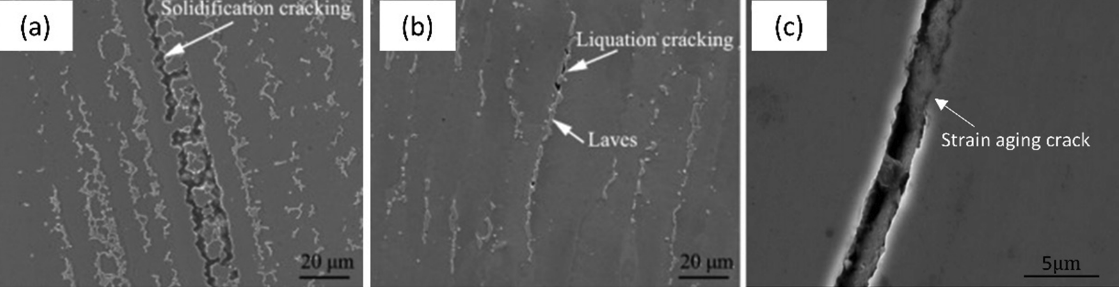
\includegraphics[width=0.8\textwidth]{Images/microstructure.png}
    \caption[Microstructure details.]{Typical microstructure details for AM part delamination and different types of AM cracking: solidification cracking (a); liquation cracking (b); strain aging cracking (c). \cite{mostafaei_defects_2022}.}
    \label{fig:microstructuredefect}
\end{figure}
\paragraph{Defect Causes.} Defect causes can be divided into four main categories:
\begin{itemize}
    \item \textbf{Defects induced by feedstock material.} Various defects could impact the metal powder used in Powder Bed Fusion (PBF), such as irregular structures of the particles, absorbed gas, and particles exhibiting satellites or fractures. Problems related to dimensions and shapes influence the powder's apparent density and flow characteristics, directly influencing the final part's quality and performance. Indeed, as we said in Section \ref{sec:metalpowders}, we can set atomization parameters to get a specific particle size range, but we cannot control it very precisely, given the nature of the process. Fig. \ref{fig:particlesdistributions} shows different particle distributions for different processes. We can reduce these defects by measuring the particle size of powder sampling before printing. We can use more straightforward methods, such as sieve analysis, or more complex procedures, such as laser diffraction or microscopy. Alternatively, as the particle distribution influences the flowability of the powder, we can measure this using the Carney funnel. Moisture, organic substances, adsorbed gases, and oxides and nitride films on particle surfaces might contaminate metallic powders. These contaminations can increase across successive cycles of powder reuse, and they could lead to a degradation of the mechanical properties of the material.
\begin{figure}
    \centering
    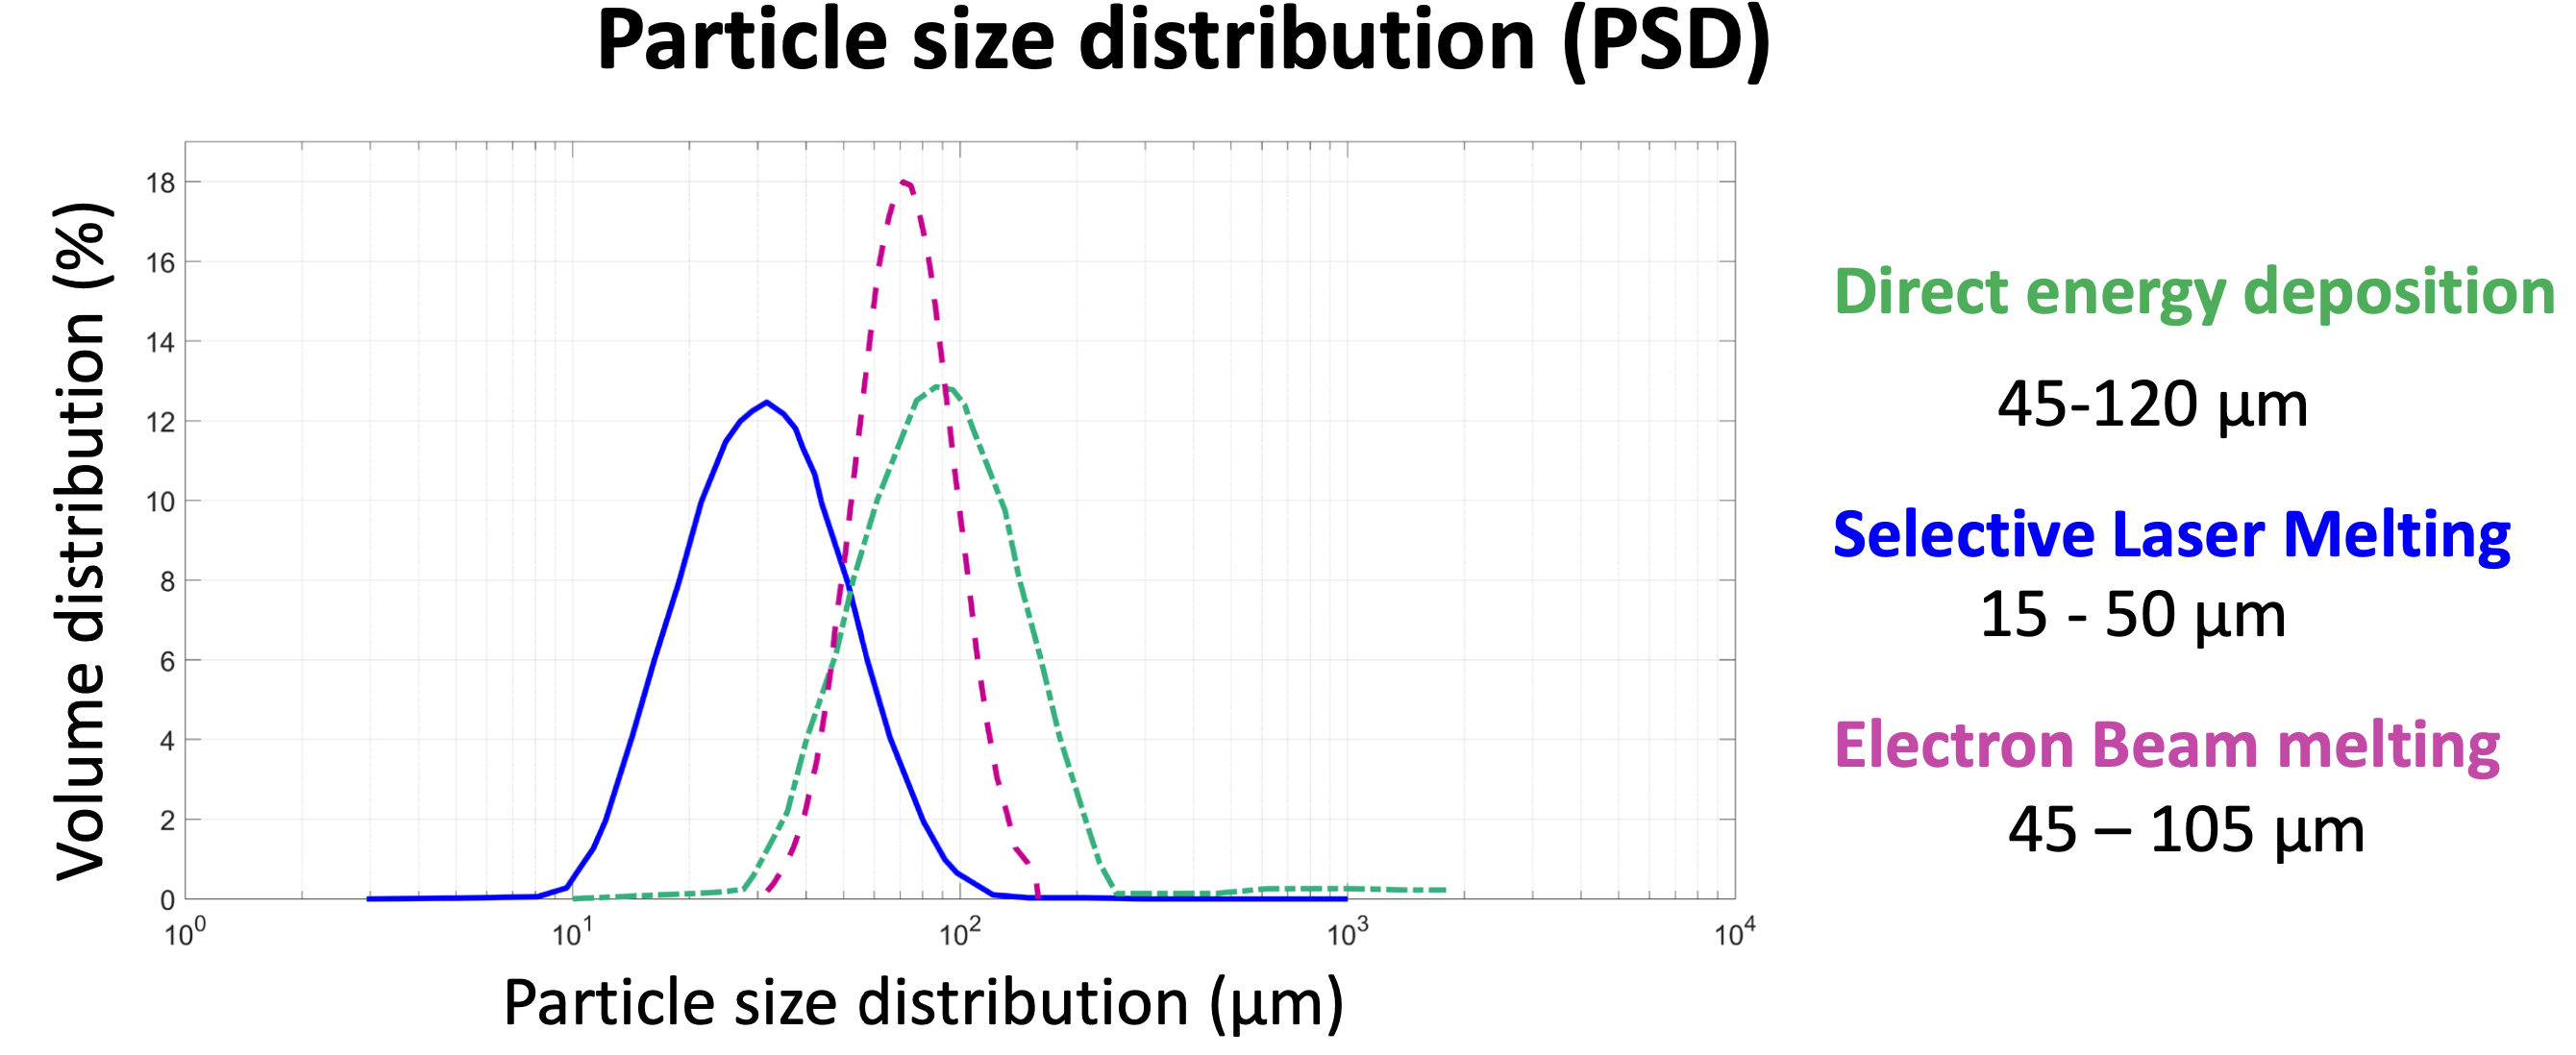
\includegraphics[width=0.75\textwidth]{Images/particlesdistributions.png}
    \caption[Particles distribution.]{Particles size distributions for different powders used in different PBF processes}
    \label{fig:particlesdistributions}
\end{figure}
    \item \textbf{Equipment-induced defects.} This category of defects results from misuse or degradation of certain critical printer parts. A classic example is the optical system of L-PBF printers or the electron gun of EB-PBF printers. Some defects are generated not only by excessive usage of these components but also by their incorrect calibration. The control of the atmosphere in the printing chamber can also give rise to defects. The flow rate and the laminarity of the inert gas in L-PBF printers directly impact the final quality, including porosity and geometrical accuracy. In addition, the oxygen inside the chamber can also interfere with the laser beam. However, the powder recoating system is one of the most critical components for this defect category. Indeed, the linear motion of the recoating system causes defects that may have been generated in other printing areas to spread all over the build area. This aspect is critical when carrying out batch production: one defective part could lead to all parts' defectiveness. Some automatic repair systems can be used in an industrial context. One example is Penelope. Penelope is an in-situ automatic defect removal prototype. Using a high-resolution chamber, a high-speed chamber, and an MWIR chamber, the system can detect super-elevated edges that could be a source of defect propagation. Once the defects have been identified using computer vision techniques, a grinding cart passes over the defective layer, selectively removing the critical areas and preventing the recoating blade from spreading the defect \cite{colosimo_penelope_2020}.
    \item \textbf{Defects due to improper design or job preparation.} Even though software tools for 3D printing have become better at helping designers make smart decisions and create optimized designs using generative techniques, many of the choices about design and printing still come from the designer's experience. Furthermore, complex objects need some trade-offs and different tries to get them right. Another cause for defects is the wrong support design. The supports are essential to stop finished pieces from warping because of thermal stress. Another possible defect source is improper part orientation within the build volume. 
    \item \textbf{Process setting–induced defects.} Printing parameters or scanning strategies often generate defects in PBF processes. Indeed, both of them depend on the part's material and design. Since almost all PBF systems only allow to set printing parameters at the beginning of the process, a trial and error approach may be necessary for particularly complex designs to obtain the proper parameter configuration. In general, it is almost impossible to achieve first-time-right production.
\end{itemize}
% <<< End of Categories of Defect in PBF Processes

%%%%%
%%%%%

% >>> Defects Monitoring Methods
\section{Defects Monitoring Methods}
\label{sec:comelotrovo}
In recent years, thanks to advancements in both available computational power at lower cost and rising technology of sensors, quality control has evolved into an increasingly complex and sophisticated process. In AM, we can collect huge amounts of data with remarkable granularity due to the layer-wise production process. This section outlines the various approaches to quality control, providing a terminology framework as established in \citeauthor{richard_leach_integrated_2020} (2020) and \citeauthor{grasso_-situ_2021} (2021).
\begin{figure}
    \centering
    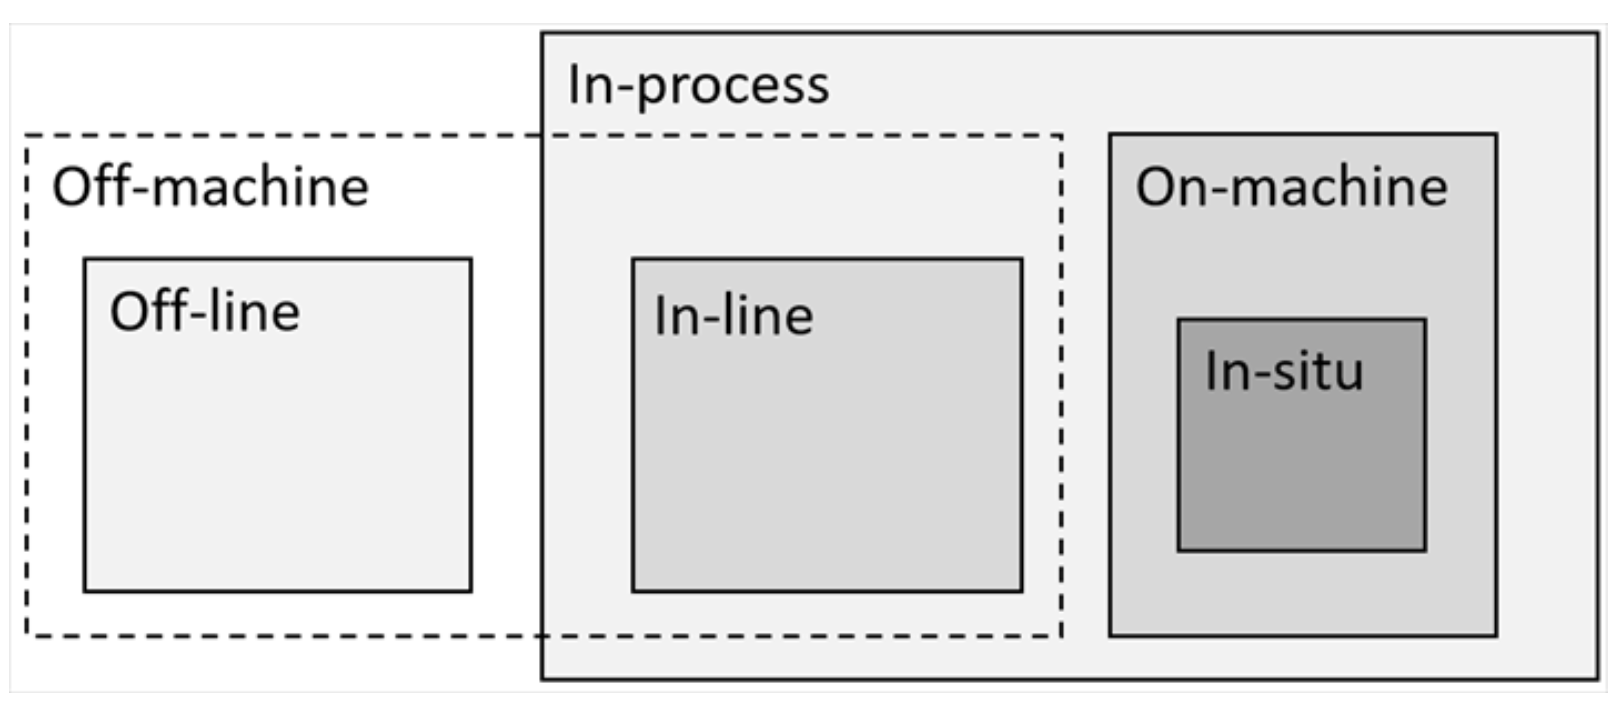
\includegraphics[width=0.6\textwidth]{Images/dovevai.png}
    \caption[Measurement and monitoring techniques.]{Graphical representation of different terms associated with measurement and monitoring techniques \cite{richard_leach_integrated_2020}.}
    \label{fig:dovevai}
\end{figure}
\emph{In-process} methods involve measuring data during or between consecutive production phases within the same manufacturing chain. These measurements are synchronized with the different stages of the manufacturing process, thus allowing monitoring them synergetically. When in-process measurements are executed immediately before, after, or amidst manufacturing points, they are called \emph{in-line} measurements. These are measured on distinct measurement systems along the standard production line, where manufacturing is not occurring. Consequently, they fall under off-machine measurements. \emph{Off-machine} measurements are taken outside the machine where the manufacturing process occurs. On the other hand, if measurements taken during the process use sensors mounted on the production machine, they are labeled \emph{on-machine} measurements. Those that principally collect data directly from the manufacturing site are called \emph{in-situ} measurements. In AM processes, in-situ predominantly denotes sensing and surveillance techniques aiming to capture details about process stability and product quality during manufacturing. Data from this last method are particularly significant as they are collected close to the final product, thus carrying out much information. When monitoring systems are not "in-process", they are labeled as off-line or \emph{"ex-situ"}. They are categorized as off-machine measurements, usually executed outside the core manufacturing setup, perhaps in a separate measurement station or a lab. Within the domain of in-situ measurements, there is a slight difference between "in-situ measurement" and "in-situ monitoring". The former implies the capability of in-situ sensors to gather aspects, aiming to understand the process or assess the product's quality attributes during production. The latter alludes to the real-time identification of discrepancies, anomalies, and OOC process conditions. They often require establishing an alert system or classification algorithm. Furthermore, considering "in-situ" measurements, depending on the measured process signature, we can distinguish five different monitoring levels \cite{grasso_-situ_2021, grasso_process_2017}. These levels are "observable signatures" only, i.e., measurable quantity. "Derived signatures" also exist. These are quantities estimated via process modeling but are beyond the scope of this thesis. Fig. \ref{fig:levels} shows levels for observable signatures.
\begin{figure}
    \centering
    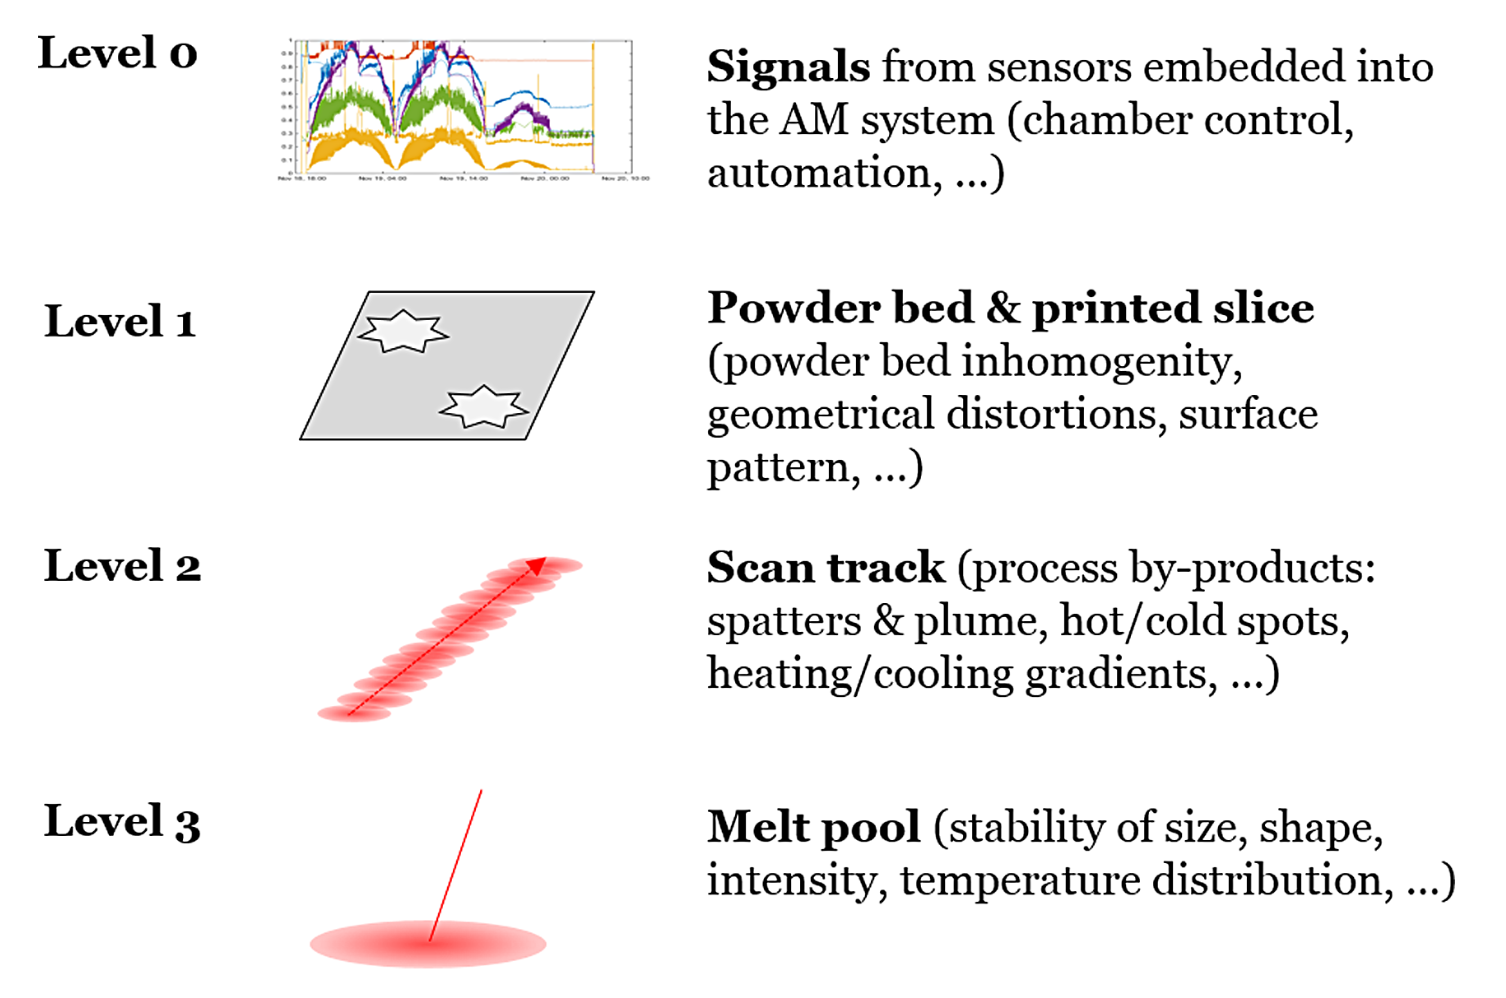
\includegraphics[width=0.8\textwidth]{Images/Level Measurement.png}
    \caption[In-situ measurement levels.]{In-situ measurement levels applicable to PBF processes \cite{colosimo_-machine_2020}.}
    \label{fig:levels}
\end{figure}
\begin{itemize}
    \item \textbf{Level 0.} At this level, we use all the signals that can be measured using embedded sensors to detect anomalies and unstable process conditions. The printer control unit usually employs these sensors to control the machine state and machine chamber environment. Indeed, the main advantage of Level 0 is the possibility of monitoring the process without needing external or additional sensors, especially in EBM printers, where many signals are already available. However, these signals are often distant from the actual process dynamics. Some examples of these signals are chamber pressure, ambient temperature, and inert gas flow.
    \item \textbf{Level 1.} This level involves measurements gathered once (or more than once) per layer of the entire build area. We are interested in both the homogeneity of the powder bed and the geometrical and dimensional features of the printed slice, and in general, all the anomalies that can be captured by using a static 2-D view of the printing plane;
    \item \textbf{Level 2.} This level includes quantities representing the process quality and stability while the beam scans the tracks within the print area. Usually, these quantities can be measured with a temporal resolution higher than the layer-wise resolution of the previous level since we can rely on sensors with high sampling rates (some cameras can use up to 10,000 fps). It is also higher than the sampling frequency of embedded sensors.
    \item \textbf{Level 3.} Process signatures at this level have the highest granularity possible in PBF systems, i.e., the melt pool. The melt pool is known to be a primary feature of interest in any process that involves a beam-material interaction aimed at achieving a local fusion of the material since it highly impacts the quality of the part and stability of the process. Some examples of process signatures are the melt-pool size, its shape, and the temperature profile of the melt pool itself;
    \item \textbf{Level 4.} This level regards the capability of gathering information about phenomena occurring under the currently processed layer. These measurements can be obtained with ad-hoc prototype machine configurations that enable transverse x-ray imaging or ultrasound and acoustic emissions caused by releasing elastic energy and plastic deformation of solidified layers. This research stream is relatively recent; indeed, it is not included in Fig. \ref{fig:levels}.
\end{itemize}
% <<< End of Defect Monitoring Methods


%%%%%
%%%%%

\section{Sensors for Defect Detection}
\label{sec:sensoriniiniini}
Each level described in Section \ref{sec:comelotrovo} involves different sensor typologies. This section describes the most widely employed sensors for in-situ process monitoring and measurement in AM. 

In \emph{level 0}, we can use embedded sensors integrated within the printer. These process signatures are particularly suitable in EB-PBF applications since many embedded systems are already mounted on EBM printers. Embedded sensor signals in EB-PBF are also known as "log signals". Publications proposed a more advanced in-process use of signals from such sensors only in EB-PBF applications as a possible source of information for in-situ anomaly detection as in \citeauthor{grasso_data_2018} (2018) and \citeauthor{steed_falcon_2017} (2017). The same publications pointed out that many of these EB-PBF log signals are correlated with process errors and variations in process conditions. \citeauthor{steed_falcon_2017} (2017) proposed a software tool for the visualization and analysis of significant multivariate time series log signals called Falcon. 

In \emph{level 1}, i.e., measurement and characterization of layer properties, we can distinguish two further types of measurements. The first is conducted before laser scanning, which allows us to identify areas where the powder bed is not uniform, potential defects produced by the recoating system, or super-elevated edges. We also can measure the laser scanning, through which we can detect any contamination of the powder of the printed slice or any geometric or dimensional deviations from the nominal shape. Several types of sensors can be employed for anomaly detection at this level.
\begin{figure}
    \centering
    \subfloat[\label{fig:offaxiallaser}]{
        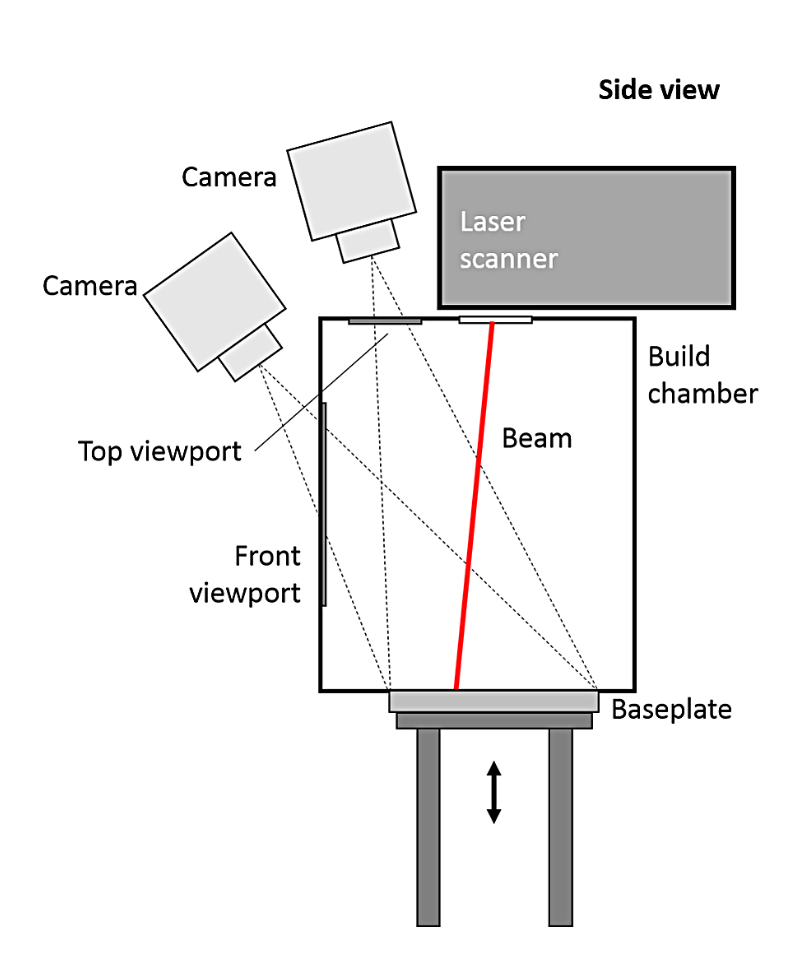
\includegraphics[scale=0.3]{Images/off axial laser.png}
    }
    \qquad
    \subfloat[\label{fig:fig:offaxialebm}]{
        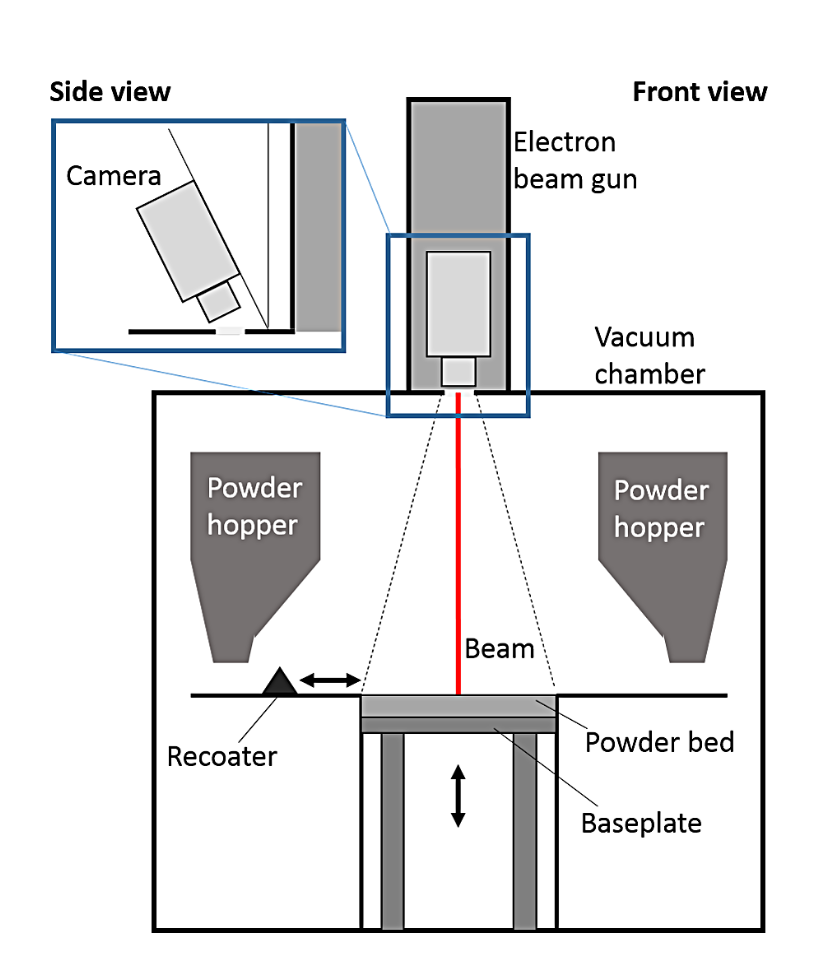
\includegraphics[scale=0.3]{Images/off axial EBM.png}
    }
    \\
    \subfloat[\label{fig:quadratoir}]{
        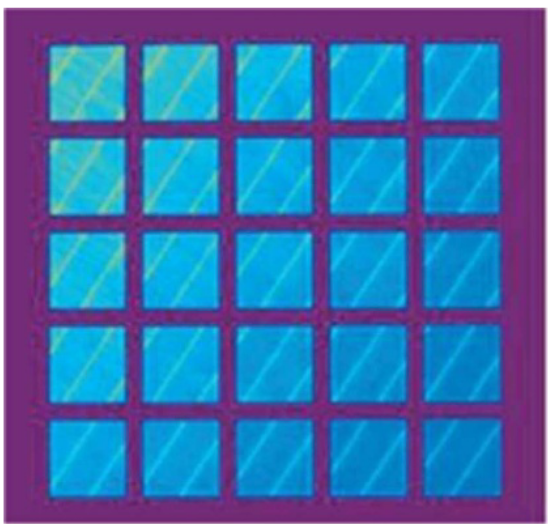
\includegraphics[scale=0.4]{Images/quadratoir.png}
    }
    \qquad
    \subfloat[\label{fig:cilindroir}]{
        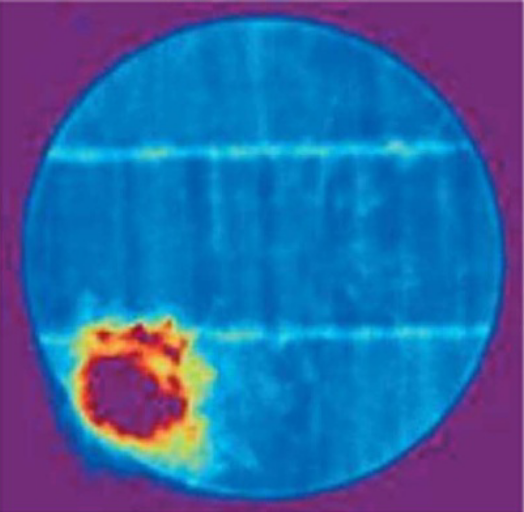
\includegraphics[scale=0.4]{Images/cilindroir.png}
    }
    \caption[Monitoring systems configurations and optical tomography examples.]{Example of off-axis sensing architectures in SLS (a) and EBM (b) \cite{colosimo_-machine_2020}, and examples of optical tomography images for cubic samples with a variation of energy density (c) and a cylinder produced under shielding gas flow variation (d)\cite{bamberg_-process_2016}.}
\end{figure}

\paragraph{Off-Axis Sensing.} In both SLS and EBM, off-axis sensing is suitable for gathering information. Conventional cameras operating in the visible range are usually employed in L-PBF (Fig. \ref{fig:offaxiallaser}), while the high temperatures in EBM and the difficulty of installing additional sensors on EB-PBF machines (Fig. \ref{fig:fig:offaxialebm}), makes their usage more challenging. The off-axis optical camera within the visible range has a significant drawback: numerous publications such as \citealt{kleszczynski_error_2012} (2012) and \citeauthor{foster_bk_optical_2015} (2015) have shown how appropriate illumination condition significantly impacts the camera's acquired result. Both the surface pattern of the printed slice and the powder bed, as well as the contrast between the background (powder) and foreground (printed slice) areas, are influenced by the intensity, nature, and relative angle of the illumination source. Hence, non-uniform illumination conditions may mask some anomalies and require some post-acquisition operations that might be challenging. The relative angle between the camera and the illumination source is also relevant in this measurement, as shown in  \citeauthor{caltanissetta_characterization_2018} (2018). Moreover, we must correct the distorted perspective given by the camera's positioning through specific geometric adjustment transformation before analysis. In addition to traditional cameras, those operating in the NIR/IR range can monitor level 1 process signatures. They are particularly suitable in EBM processes due to the high temperatures encountered during printing. Fig. \ref{fig:quadratoir} and Fig. \ref{fig:cilindroir} show two examples of acquired images. 
\begin{figure}
    \centering
    \subfloat[\label{fig:fringesetup}]{
        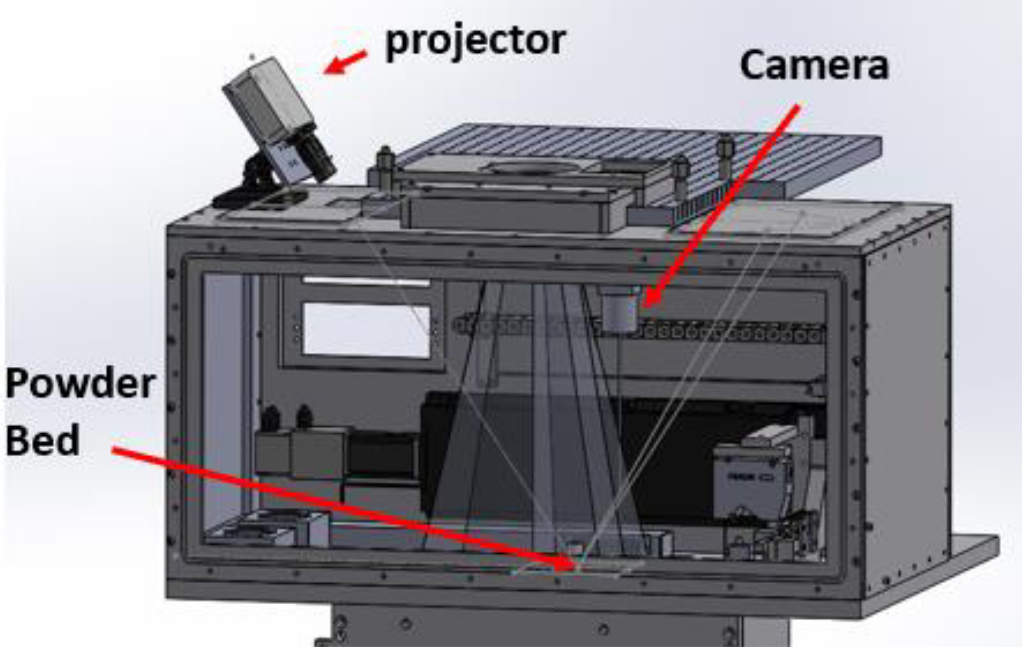
\includegraphics[scale=0.35]{Images/fringesetup.png}
    }
    \qquad
    \subfloat[\label{fig:fringeprojection}]{
        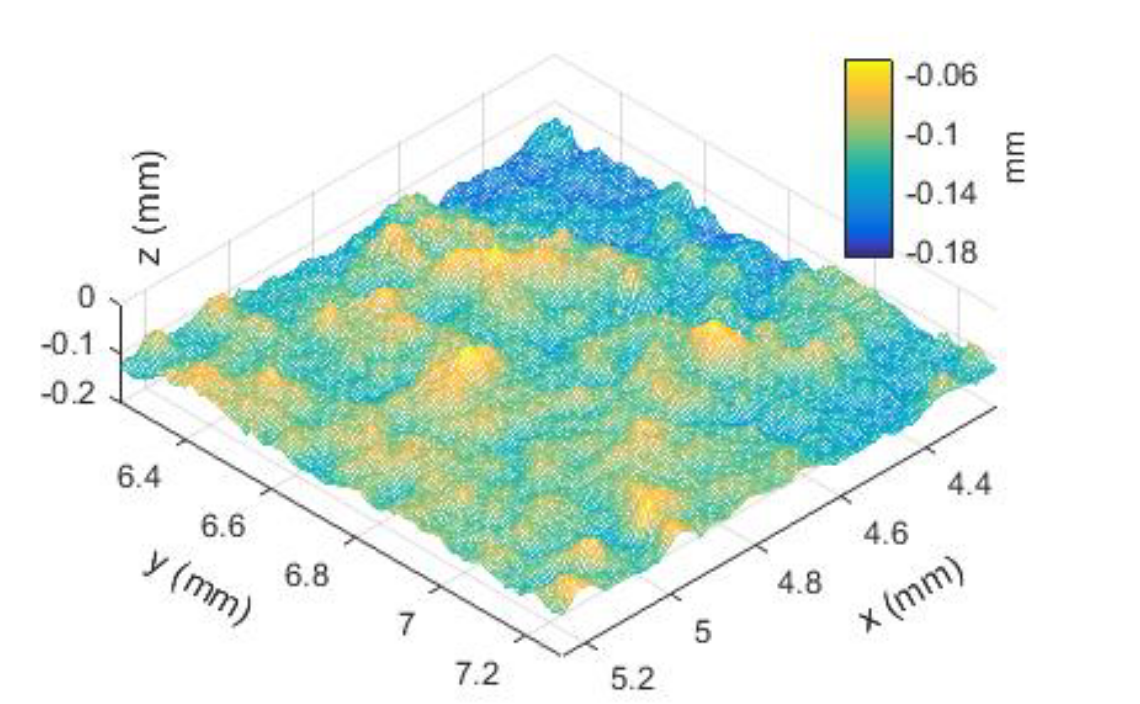
\includegraphics[scale=0.35]{Images/fringeprojection.png}
    }
    \caption[Fringe projection.]{Setup for fringe projection measurement system (a) and reconstructed height map of the power bed (b) \cite{zhang_situ_2016}.}
\end{figure}
One of the most employed systems for this kind of measurement is "LayerQam", developed by Arcam (GE Additive) for integration in its EB-PBF machines. The system consists of an NIR camera that acquires an image of the layer after the melting phase and uses local pixel intensity variations to detect anomalies. Finally, bright spots are a proxy for possible volumetric flaws and material discontinuity defects.
\paragraph{Fringe Projection.} The off-axis imaging techniques mentioned in the preceding paragraph can generate a 2D reconstruction of the powder bed and the printed section. We can achieve a height map, a 3D representation of the powder bed, with fringe projection. We need to merge the visualization layer with topographic examination to achieve this map. The standard configuration for such measurements consists of a camera (single-view configuration) and a projector. Fig. \ref{fig:fringesetup} shows a typical system configuration, while Fig. \ref{fig:fringeprojection} shows an example of a height map.
Other authors proposed and tested multi-view configurations with two or more cameras, suitable for higher resolution and accuracy \cite{kalms_new_2019}.
\begin{figure}
    \centering
    \subfloat[\label{fig:coaxiallaser}]{
        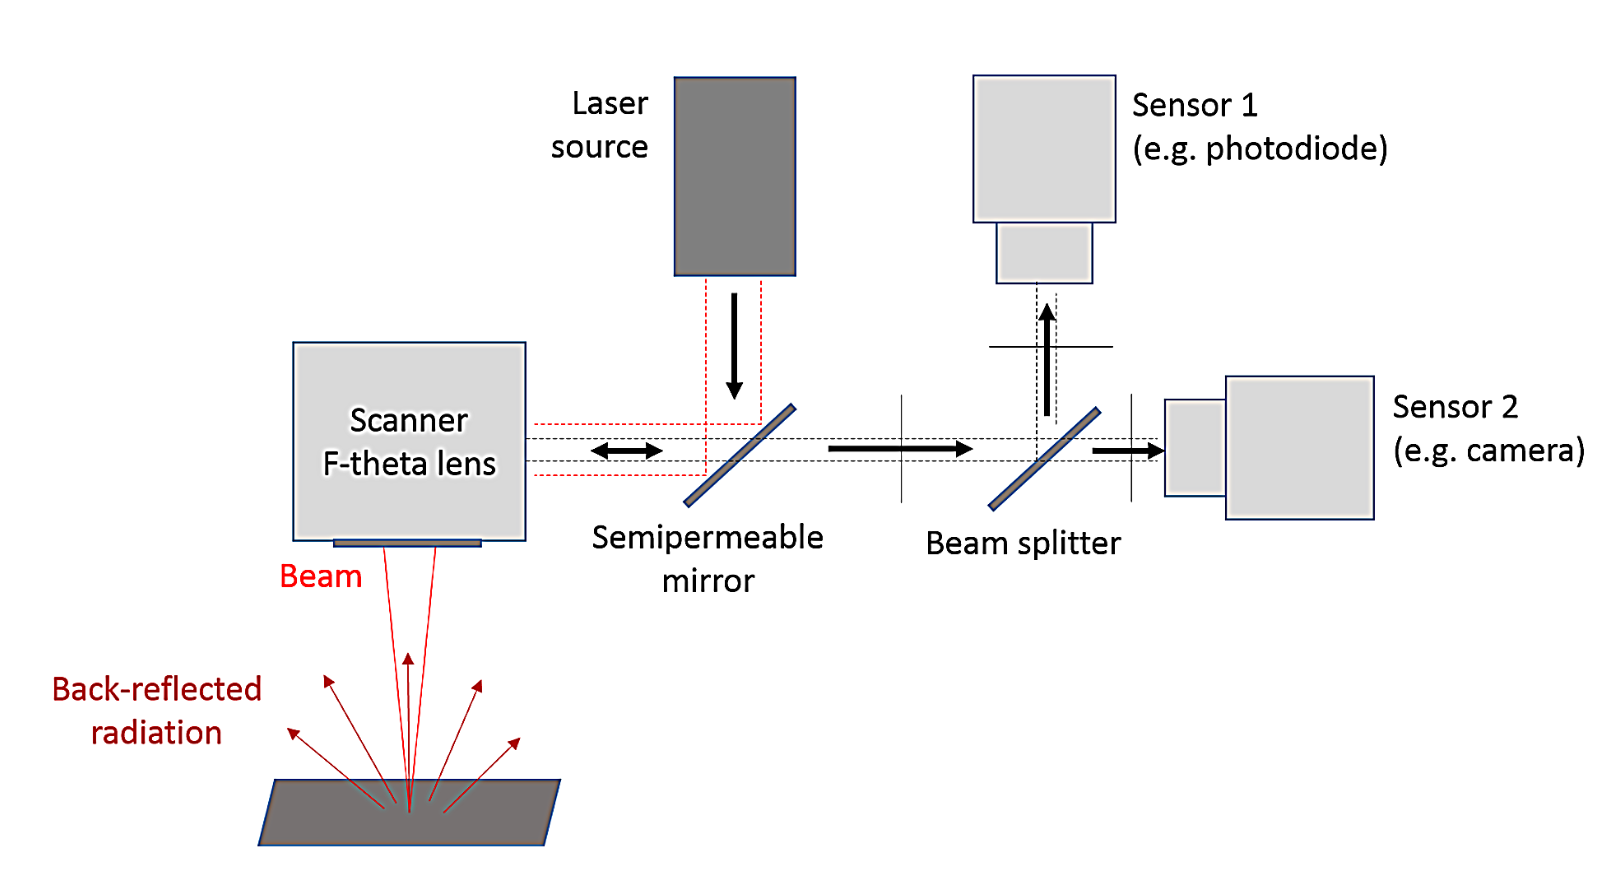
\includegraphics[scale =0.35]{Images/coaxial laser.png}
    }
    \qquad
    \subfloat[\label{fig:coaxialheatmap}]{
        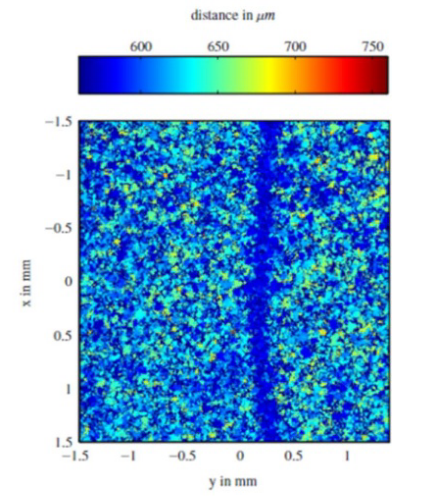
\includegraphics[scale=0.5]{Images/coaxialmap.png}
    }
    \caption[Co-axial sensing and results.]{A graphical representation of a system for co-axial sensing in L-PBF \cite{colosimo_-machine_2020} (a) and a corresponding in-situ topography reconstruction (b) \cite{neef_low_2014}.}
\end{figure}
\paragraph{Blade Mounted Sensor.} Another possible approach for level 1 process monitoring is to employ an optical sensor directly mounted on the recoating blade of PBF printers. By doing so, we can avoid the geometric distortion typical of off-axis systems. Moreover, these sensors can obtain a 2D representation of the print bed and reconstruct the height map. In the former case, we can get a resolution up to \SI{4800}{DPI} over a length of \SI{210}{\milli\metre} with a spatial resolution of \SI{5.3}{\micro\metre / pixel} \cite{tan_phuc_high-resolution_2019}, while in the latter we can reach a little lower resolution of \SI{20}{\micro\metre / pixel} \cite{barrett_micron-level_2018}.
\paragraph{Co-axial sensing.} L-PBF can leverage the back-scattered light from the melt pool and its adjacent areas to gauge specific metrics indicative of melt-pool dynamics. Scattered light passes through the optical path of the laser, passing the same lenses of the processing laser, and a semi-reflective mirror redirects the laser beam to the scanner while simultaneously allowing the light emitted from the melt pool to be detected by sensors. This emitted light is then divided and directed to each sensor. Various co-axial detection designs might encompass multiple pyrometers, bi-wavelength or multi-wavelength, and assorted imaging devices in the visible or infrared spectrum. Fig. \ref{fig:coaxiallaser} shows a typical co-axial sensing system. With this method, we can reach high sample rates of \SI{50}{\kilo\hertz}, but the observation area is typically limited to \qtyproduct{0.5 x 0.5}{\milli\metre}, making this method unsuitable to capture time evolution of the physical phenomenon. Alterations in the melt pool's dimensions and luminosity/temperature can induce changes in the pyrometer's readings, facilitating the observation of melt pool consistency and any unusual signal shifts. This architecture was first developed by the Katholieke Universiteit Leuven and licensed by Concept Laser \cite{colosimo_-machine_2020, kruth_jean-pierre_feedback_2007, berumen_quality_2010}. This measurement approach has achieved outstanding results, with a lateral resolution of \SI{30}{\micro\metre} and a vertical resolution of \SI{7}{\micro\metre} \cite{fleming_tracking_2020}.

\paragraph{Electronic imaging.} In EBM, the process gives rise to by-products like secondary and back-scattered electrons and x-rays. The electrons generated from the beam and metal powder interaction could be harnessed and used to produce an electronic representation of the layer. Thus, one of the undesired effects outlined in Section \ref{sssec:electroninteractions} can be leveraged to extract valuable insights about the current state of the process. Using only back-scattered electrons, \citeauthor{wong_pilot_2019} (2019) were able to reach a spatial resolution of \SI{60}{\micro\metre / pixel}. Fig. \ref{fig:electronic1} shows an example of acquired images. Moreover, we can use an electron beam to scan the layers and metal surfaces, using the heat shield as an electron collector during the melting phase as done by \citeauthor{arnold_operando_2020} (2020). This approach has achieved a resolution of \numrange[range-phrase=--]{50}{100}\unit{\micro\metre / pixel}. Fig. \ref{fig:electronic2} shows an image from the study.
\begin{figure}
    \centering
    \subfloat[\label{fig:electronic1}]{
        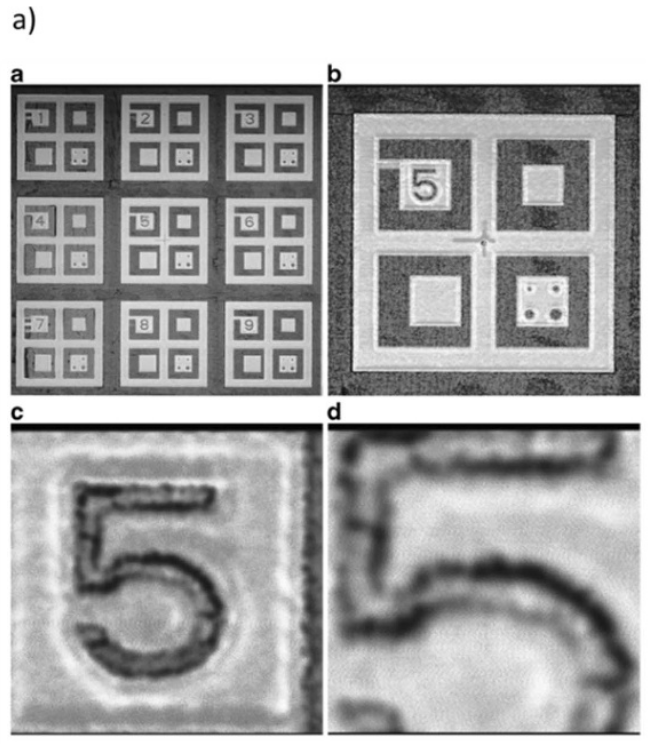
\includegraphics[scale=0.44]{Images/electronic1.png}
    }
    \qquad
    \subfloat[\label{fig:electronic2}]{
        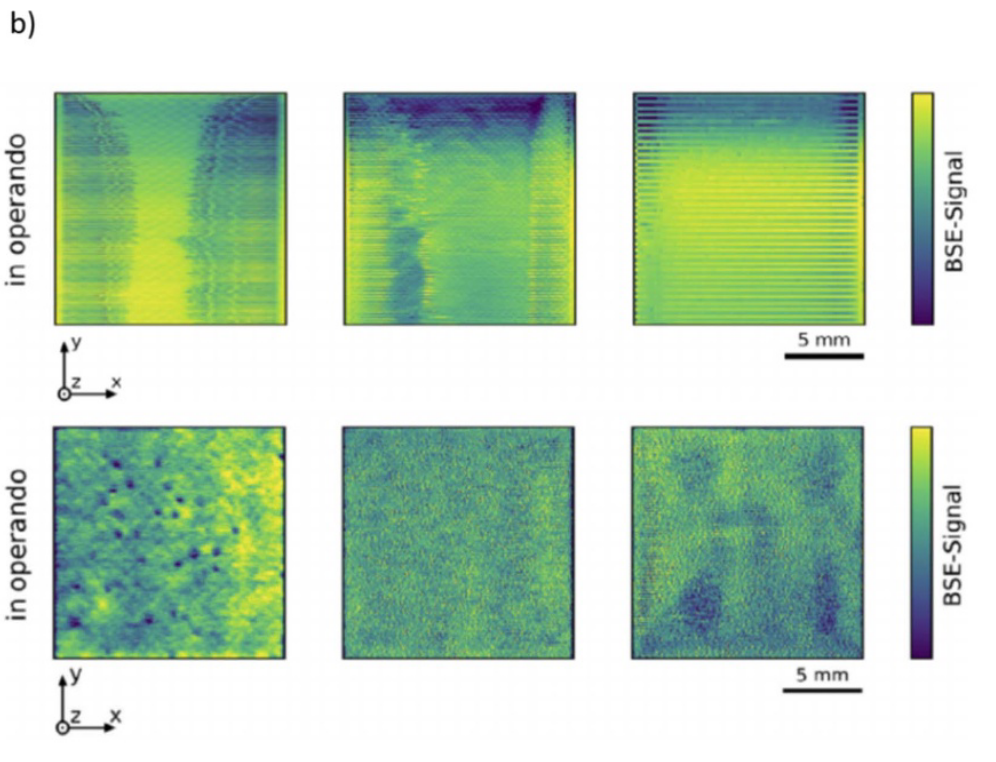
\includegraphics[scale=0.44]{Images/electronic2.png}
    }
    \caption[Co-axial sensing result.]{Examples of electronic images in EBM: images with different magnification factors (a) \cite{wong_pilot_2019} and images of squared printed areas generated via real-time back-scattered signal acquisition from different materials and with increasing hatch spacing \cite{arnold_operando_2020}.}
\end{figure}

For \emph{level 2} signatures, we use sensors for in-process measurement of fast transient phenomena and high-speed emissions during laser or electron beam scanning. The main goal of this level is to understand underlying physical phenomena that lead to the formation of the defect. Most methods used at this level involve off-axis mounted sensors, mainly cameras in the visible range or thermal cameras with high temporal resolution. Indeed, this is needed to capture fast and transient phenomena. 
\paragraph{Measurement of Process Heatmap and Temperature Profiles.} We will address this paragraph with greater detail as these methods detect the defects discussed in Section \ref{sec:hotspot}.
\begin{figure}
    \centering
    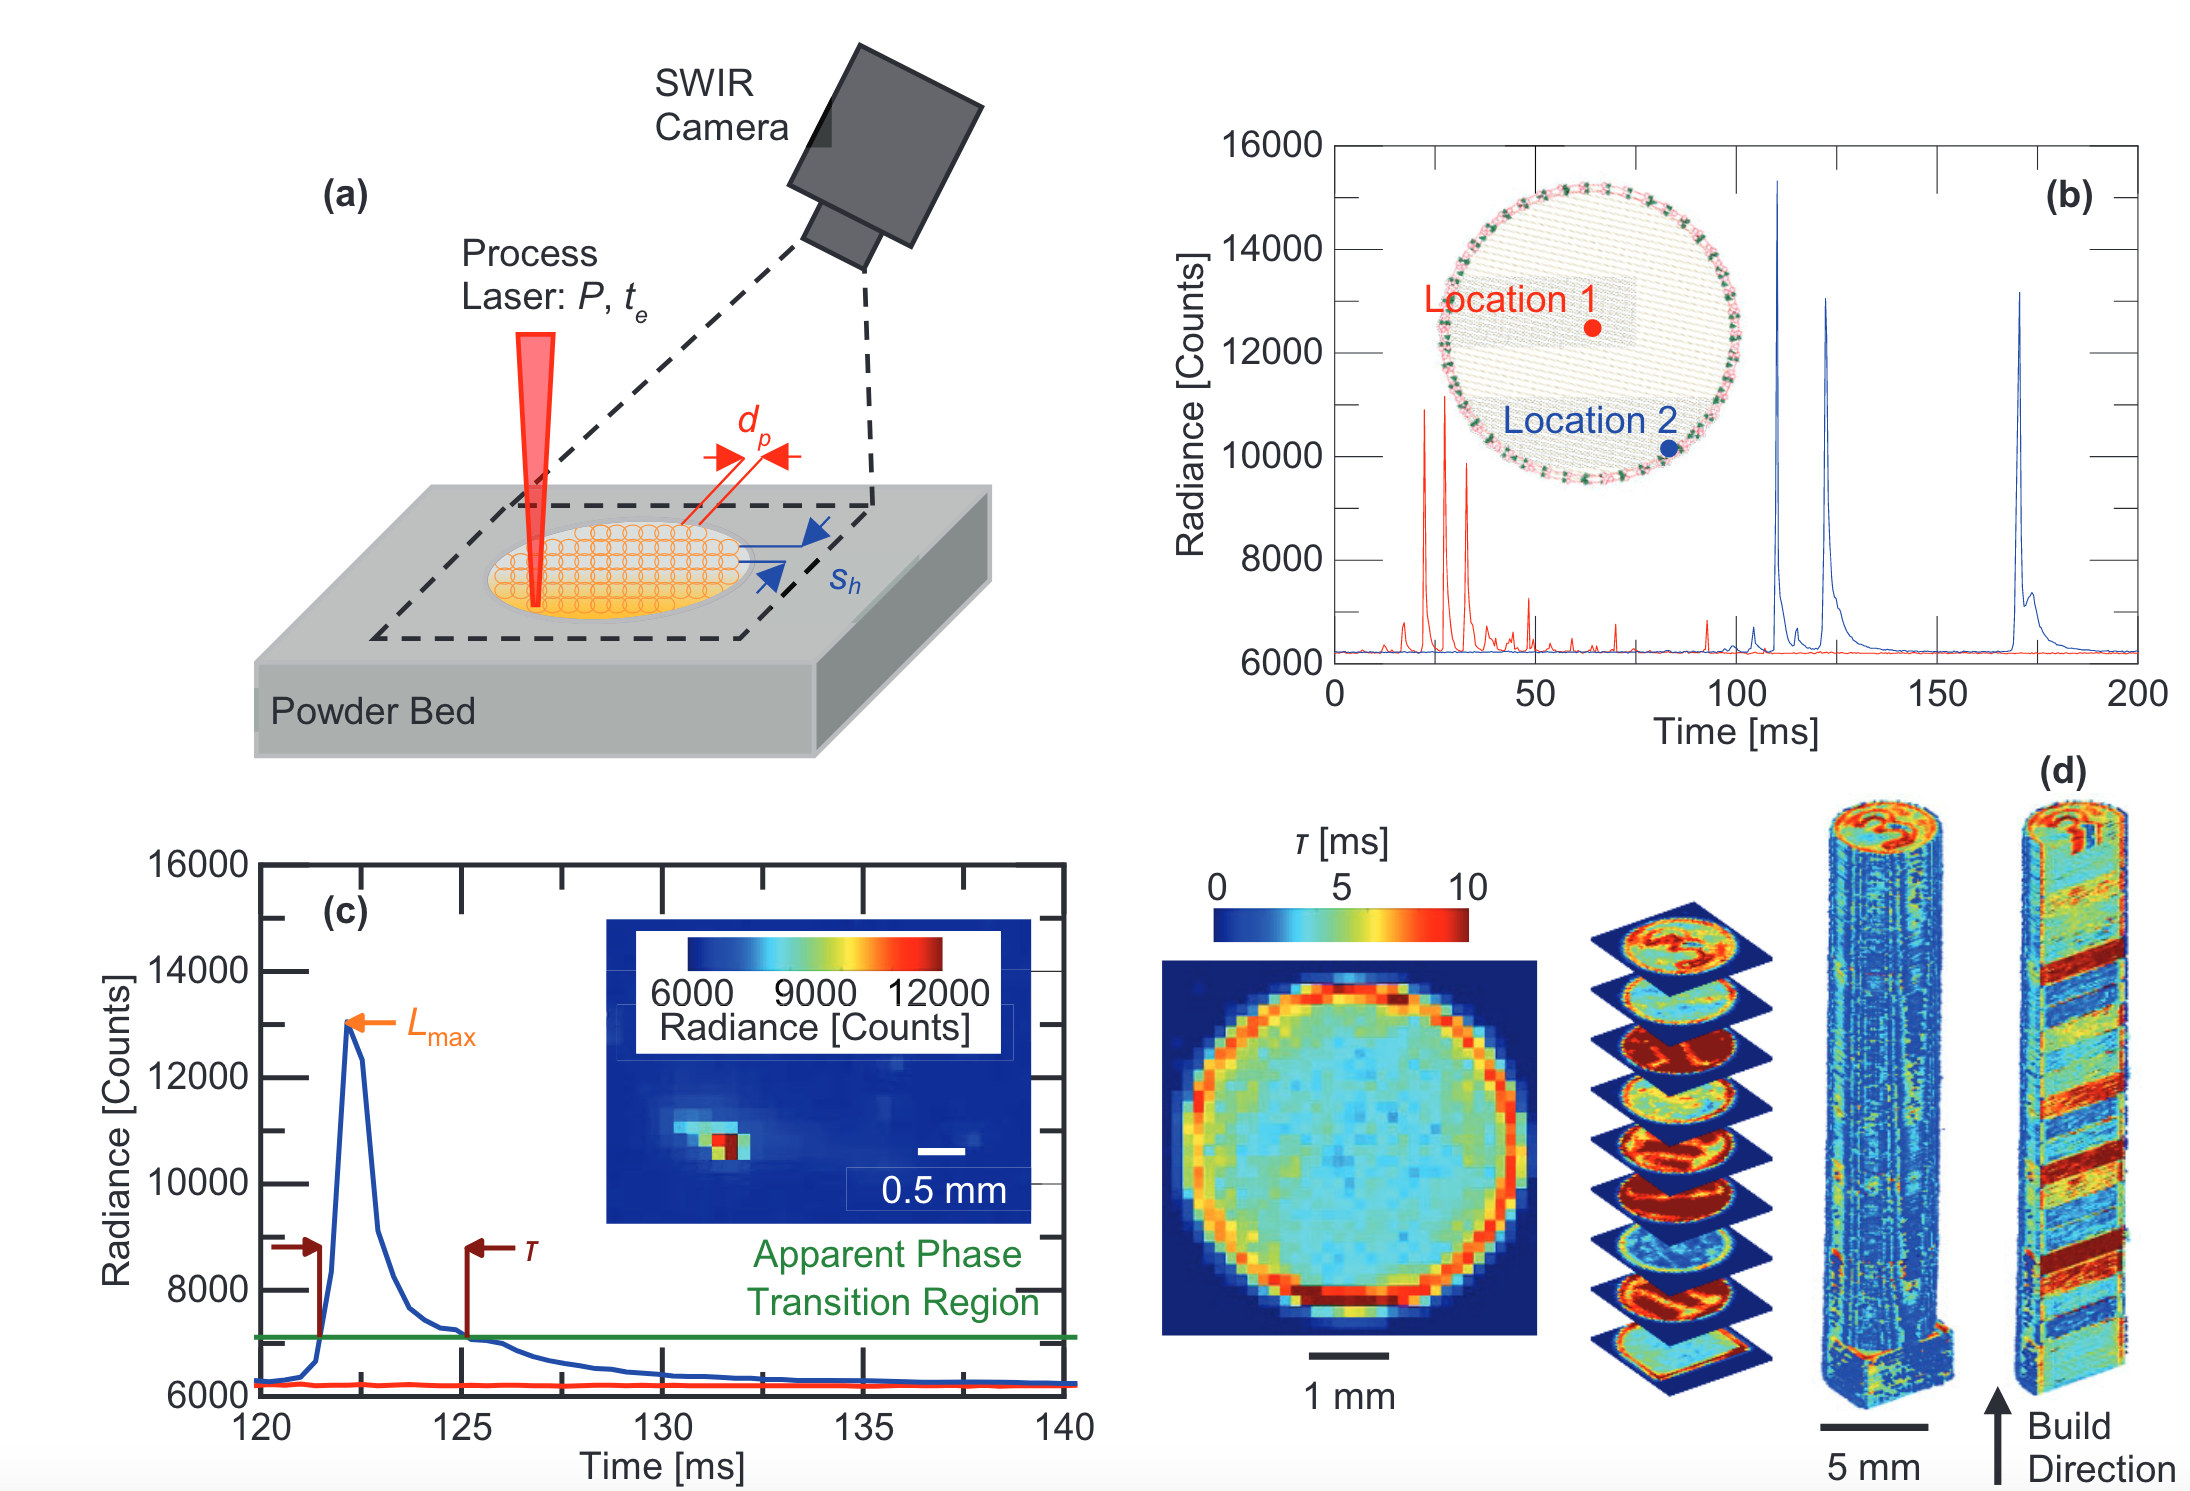
\includegraphics[width=0.8\textwidth]{Images/voxel.png}
    \caption[Example of voxel thermic reconstruction.]{(a) SWIR camera observation of SLM process, (b) time series data from a location in the center of part cross-section (location 1) and border scan region (location 2), (c) definition of thermal features in time series data with melt pool image, and (d) thermal feature maps showing generation of volumetric data and slicing \cite{lough_-situ_2019}.}
    \label{fig:voxel}
\end{figure}
The layerwise manufacturing paradigm allows the "seeing" of the thermal history of the process in a new dual-paradigm. In this new paradigm, time and space overlap over the z-axis. Indeed, the production of an object using additive manufacturing grows in the same direction over time and space. \citeauthor{williams_situ_2019} (2019) demonstrated that almost all major quality characteristics of the final part and its mechanical performance depend on the thermal history. Local and global variations of heating and cooling patterns may affect material solidification at volumetric, microstructural, and geometrical levels. We can identify two primary goals linked to this monitoring system. The first focuses on building a heatmap of the layer using data collected at slower rates (up to 50 fps), and the other targets recording rapid thermal fluctuations, with time resolutions ranging from \numrange{300}{10000} \unit{fps}. In terms of spatial resolution, we can use measurement setups with a limited field of view, which enable us to resolve \numrange[range-phrase=--]{8}{100}\unit{\micro\metre / pixel}, or with a field of view covering the entire build area, with a resolution typically above \SI{100}{\micro\metre / pixel}. In both L-PBF and EBM, we can use thermal cameras in either short, medium or long-wave IR. To minimize measurement errors caused by the laser's light emissions, we should use a short wave IR camera, with a bandwidth from \numrange{1.35}{1.6}\unit{\micro\metre} \cite{heigel_situ_2020}. \citeauthor{lough_-situ_2019} (2019) used this type of camera, and they obtained a thermal map of a specimen printed with L-PBF. Then, using extracted features from the map, they achieved a voxel-based representation of the part associated with its local and global quality attributes. Fig. \ref{fig:voxel} shows the reconstruction of the specimen. Other researchers have employed high temporal resolution IR video imaging in L-PBF to improve the ability to map temperature profiles spatially and temporally, capturing quick and transient events. Although they exhibit a high sensitivity to emissivity values when determining absolute temperatures, thermal cameras in the medium or long-wave IR spectrum can be adjusted over a broader temperature span than short-wave IR cameras. They maintain high sensitivity even at elevated temperatures, which makes them particularly suitable for in-situ thermal video imaging in EB-PBF applications, especially when we need a larger field of view to construct a thermal map. In EB-PBF, the methodologies for in-situ video imaging have to be tailored to the unique aspects of the process. Both standard and thermal imaging devices must be shielded against X-ray emissions and metal deposition. We can use X-ray shielding glass and a rotating Kapton film to protect sensors, ensuring that metallic vapors don't settle on the glass. The Kapton film allows for approximately 79\% IR transmission, while a \SI{10}{\milli\metre} x-ray shielding window lets through around 1.08\% of IR, as noted by \citeauthor{ralph_b_dinwiddie_thermographic_2013} (2013).PBF processes experience rapid state changes, transitioning from powder to a liquid state and then to a solidified form. The fast transitioning, combined with ongoing alterations in surface attributes and vaporized material emissions, could affect the accurate estimation of temperature measurements. Luckily, most of the time, we are interested more in the thermal signature fluctuation over time rather than pinpointing an absolute temperature. Data analysis and monitoring algorithms can be employed directly on original signals in these cases. On the other hand, if we need a precise temperature value, we can use more advanced thermal cameras, even if they are bigger, costly, and generally need machinery modification and viewports for mounting in working setups. Standard cameras are more cost-effective and straightforward to incorporate, and with the right equipment, they can offer high temporal precision. Even though they don't grant precise temperature assessments, variations in pixel brightness in the visible spectrum can be used as a proxy to measure thermal shifts to spot abnormalities and imperfections. 
\paragraph{Process By-Products Measurement.} Due to the different nature of the interactions in the SLS and EBM processes, as already described in \ref{sec:matterint}, we need to distinguish between the measurement systems of the by-products of these two processes. Since we have already discussed the measurement of the by-products of EBM in level 1, in this paragraph, we will focus on L-PBF processes. It has been widely demonstrated that the partial vaporization of the metal, also called plume, and the spatter ejected together with it are correlated with detrimental effects on part quality. Indeed, intense emissions of these by-products could lead to the deflection and partial absorption of the laser beam, resulting in a change of laser spot geometry or energy density drops. Fig. \ref{fig:plume} visually represents this phenomenon. We can use visual and IR video imaging techniques to obtain information about spatter and plume. In Fig. \ref{fig:colosimoplume}, we can see an example of an in-control plume generation phenomenon acquired using an IR camera. Recent research has introduced a high-speed stereo vision system to identify and trace individual spatters in the 3D space above the layer. Through this approach, it's possible to monitor the trajectory of spatters, allowing for the calculation of both their speed and their spatial-temporal behaviors. Tracking the spatter along its trajectory can enhance the understanding of process by-products, offering further clarity regarding their formations and the effect of processing conditions. We can use a high-speed, high-energy X-ray video imaging system to follow the spatter's origination mechanism.
\begin{figure}
    \centering
    \subfloat[\label{fig:plume}]{
    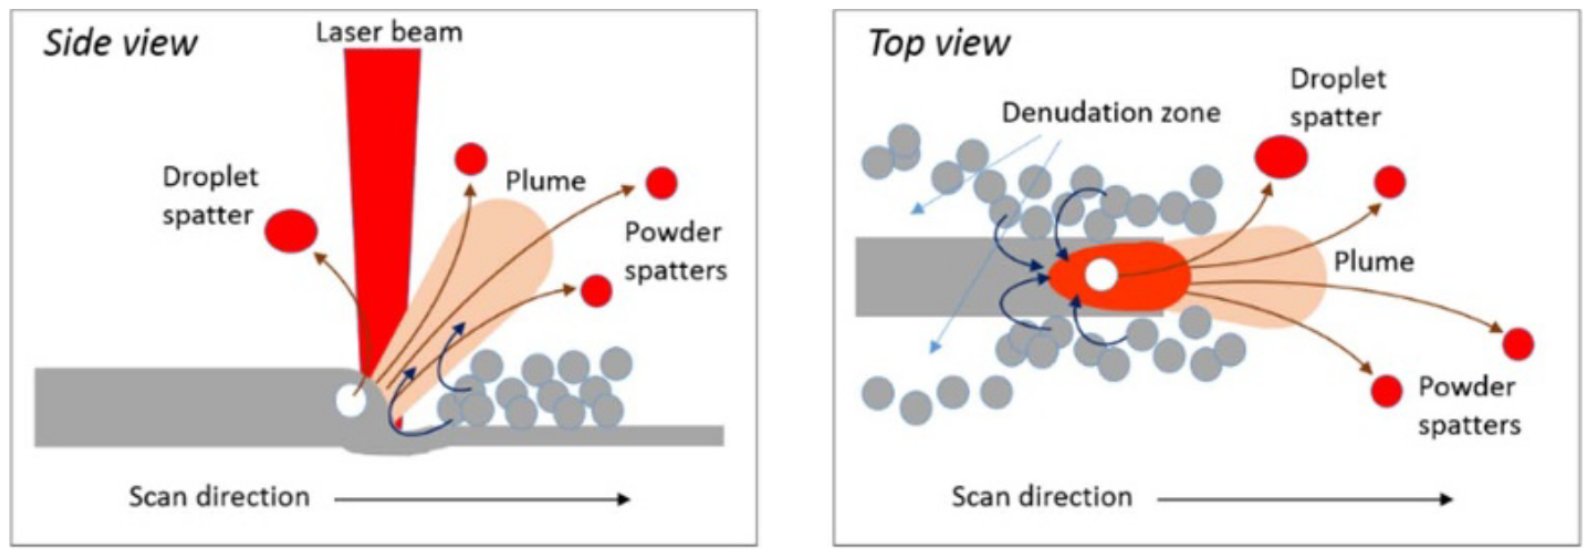
\includegraphics[scale = 0.4]{Images/plume.png}}
    \qquad
    \subfloat[\label{fig:colosimoplume}]{
        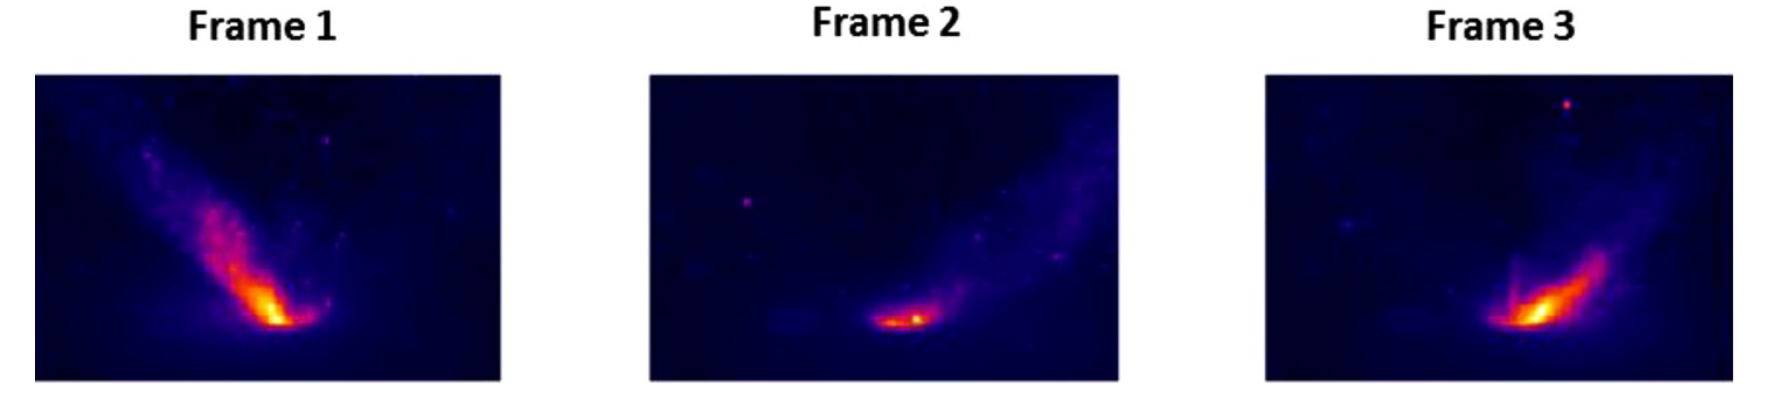
\includegraphics[scale=0.4]{Images/plumecolosimo.png}
    }
    \caption[Spatters and plume in SLS]{Schematic representation of spatters and plume emission in SLS (a) \cite{grasso_-situ_2021}, and plume emissions captured with long wave IR video imaging (b) \cite{grasso_statistical_2019}.}
\end{figure}
\paragraph{Measurement of air-borne acoustic emission.} In L-PBF processes, a research stream involves air-borne acoustic emission sensors. The measurement system captures air density variations during the laser scanning by placing the sensor near the melted area. To measure acoustic vibration, we can use a Bragg grating opto-acoustic sensor installed into the build chamber at about \SI{200}{\milli\metre} from the process zone, with a sampling frequency of \SI{1}{\mega\hertz}. In \citeauthor{wasmer_situ_2019} (2019), the sensor was placed so that the fiber's longitudinal axis was perpendicular to the acoustic wave to increase sensitivity. The result of the study can be seen in Fig. \ref{fig:acustic}. We can appreciate how different levels of porosities correspond to different audio spectra. We can also use more common sensors like in \citeauthor{ye_defect_2018} (2018). In the study, authors installed a microphone into the build chamber at an angle of \ang{30} above the build area, with a frequency response in the range \numrange[range-phrase=--]{0}{100}\unit{\kilo\hertz}. The resulting measurements and their information content in the temporal and frequency domain can be viewed as signatures of the laser-material interaction.

The melt pool carries much information since it is the phenomenon with the highest granularity possible in PBF. Melt pool properties are process signatures of \emph{level 3}. These systems have primarily been explored in L-PBF since co-axial sensors can be easily employed. Indeed, co-axial sensing is prevalently employed at this level. Using off-axis video imaging, we have already discussed some level 2 methods in EBM to extract details at both the track and melt pool levels. Recently, there's been emerging research focused on analyzing melt pool data using machine learning methods. We can identify two primary measurement systems: methods that integrate over space and resolve spatial details.
\begin{figure}
    \centering
    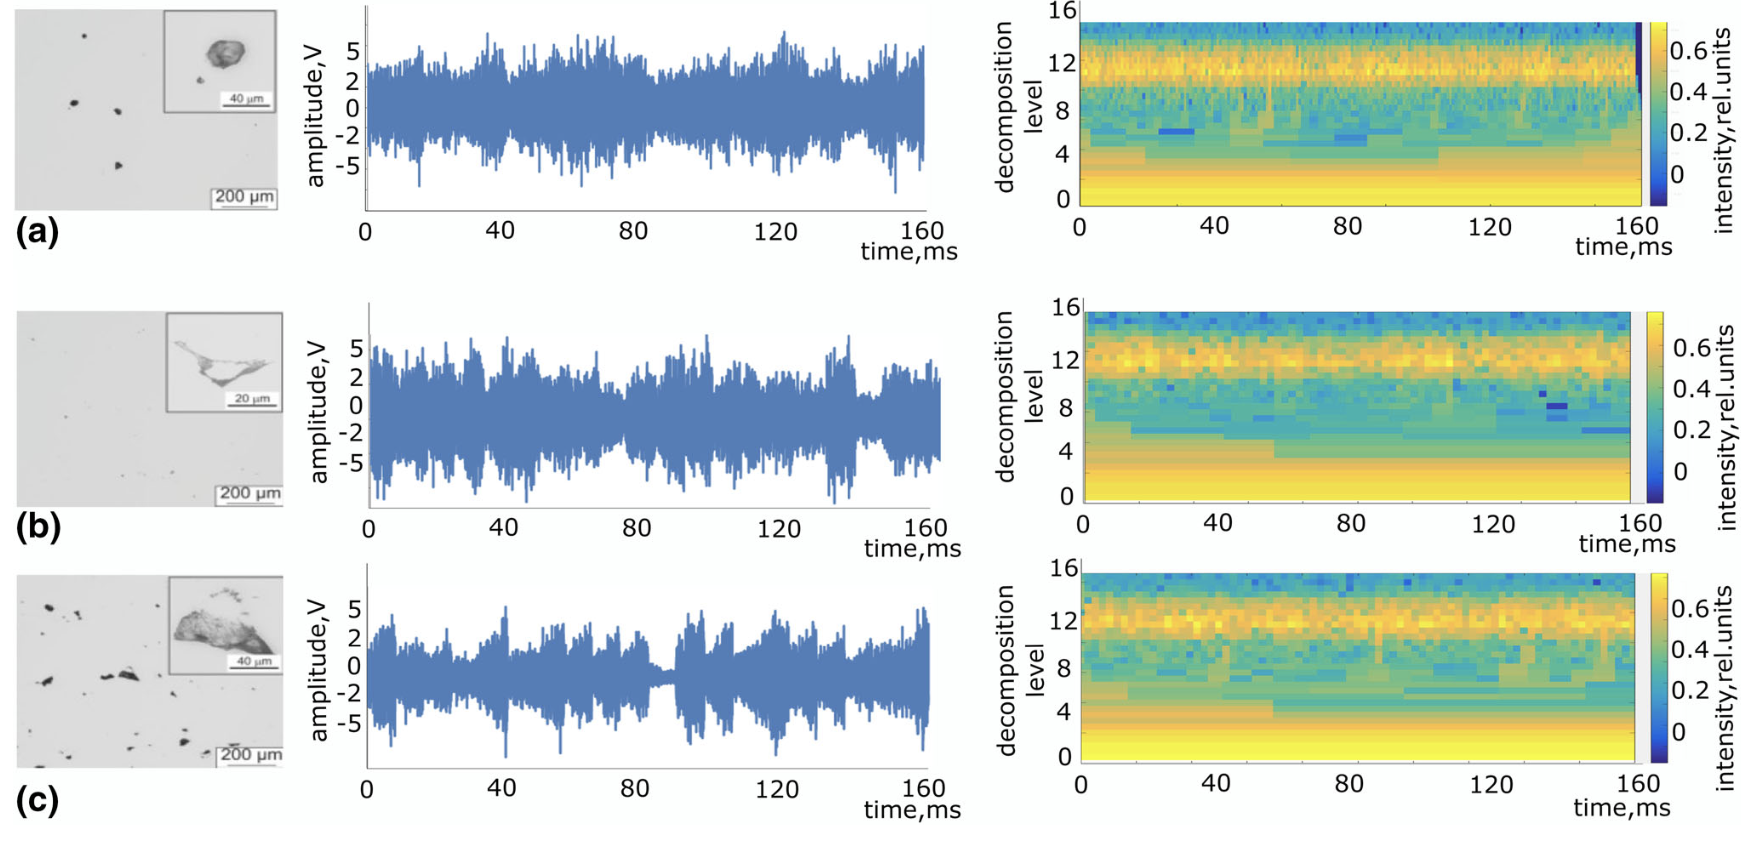
\includegraphics[width = 0.8\textwidth]{Images/acustic.png}
    \caption[Example of AE of different porosities specimens.] {From left to right, typical light microscope cross-sectional images with different porosities, their corresponding acoustic emission signals with a \SI{160}{\milli\second} time span, and their corresponding wavelet spectrogram of the regions produced with different scanned velocity \SI{300}{\milli\metre / \second} (a), \SI{500}{\milli\metre / \second} (b) and \SI{800}{\milli\metre /\second} (c) \cite{wasmer_situ_2019}}
    \label{fig:acustic}
\end{figure}
\paragraph{Spatially integrated methods.} Real-time co-axial monitoring of melt pool attributes has been employed since 2010. At this level, process signatures are the melt pool's size, shape, and the intensity and spectrum of emitted radiation. We can use spatially integrated pyrometry with single or multiple photodiodes to capture the power of radiation from the melt pool with impressive temporal accuracy, typically at a \SI{100}{\kilo\hertz} sampling rate. Acquired data quality depends on the spectral range of measurement and the sensor's field of view. Most sensors work within a range of \numrange{400}{1100} \unit{\nano\metre}, even if it's hard to find sensors for wavelengths beyond \SI{1000}{\nano\metre}. Today, co-axial photodiodes are equipped in the majority of industrial L-PBF setups. In a certain way, they are slowly becoming embedded sensors of level 0. \citeauthor{montazeri_-process_2018} (2018) showed that the chemical composition of the material could be determined via melt pool radiation measurement, finding a way to detect potential powder contaminations by analyzing spectral data. \citeauthor{lough_-situ_2020} (2020) achieved similar results using a co-axial optical emission spectroscope to capture the spectral data and infer the chemical composition of vaporized by-products. There are also sensors with larger fields of view, up to the entire build area, which enables measuring radiation emitted by surrounding hot spots. However, these sensors have a much lower resolution, not even comparable to co-axial sensors.
\paragraph{Spatially resolved methods.} Co-axial video imaging techniques can obtain more detailed insights into the melt pool's attributes and consistency over time. Commonly, a high-speed camera (\numrange{1000}{50000} \unit{fps}) paired with a narrow-band NIR filter is utilized to maximize the dynamic range and record the primary melt pool emissions. In some cases, it is also possible to use off-axis video imaging methods, using high-magnification optics combined with a limited field of view. In \citeauthor{lane_measurements_2020} (2020), the authors employed an off-axis high-speed camera paired with a mirror, facilitating an up-close examination of the melt pool without interfering with the laser beam. They achieved a spatial resolution \SI{3}{\micro\metre / pixel}. In the same paper, the authors also used a thermal camera for melt pool thermography and achieved a lower resolution of \SI{36}{\micro \metre / pixel}.
\begin{figure}
    \centering
    \subfloat[\label{fig:colorini}]{
        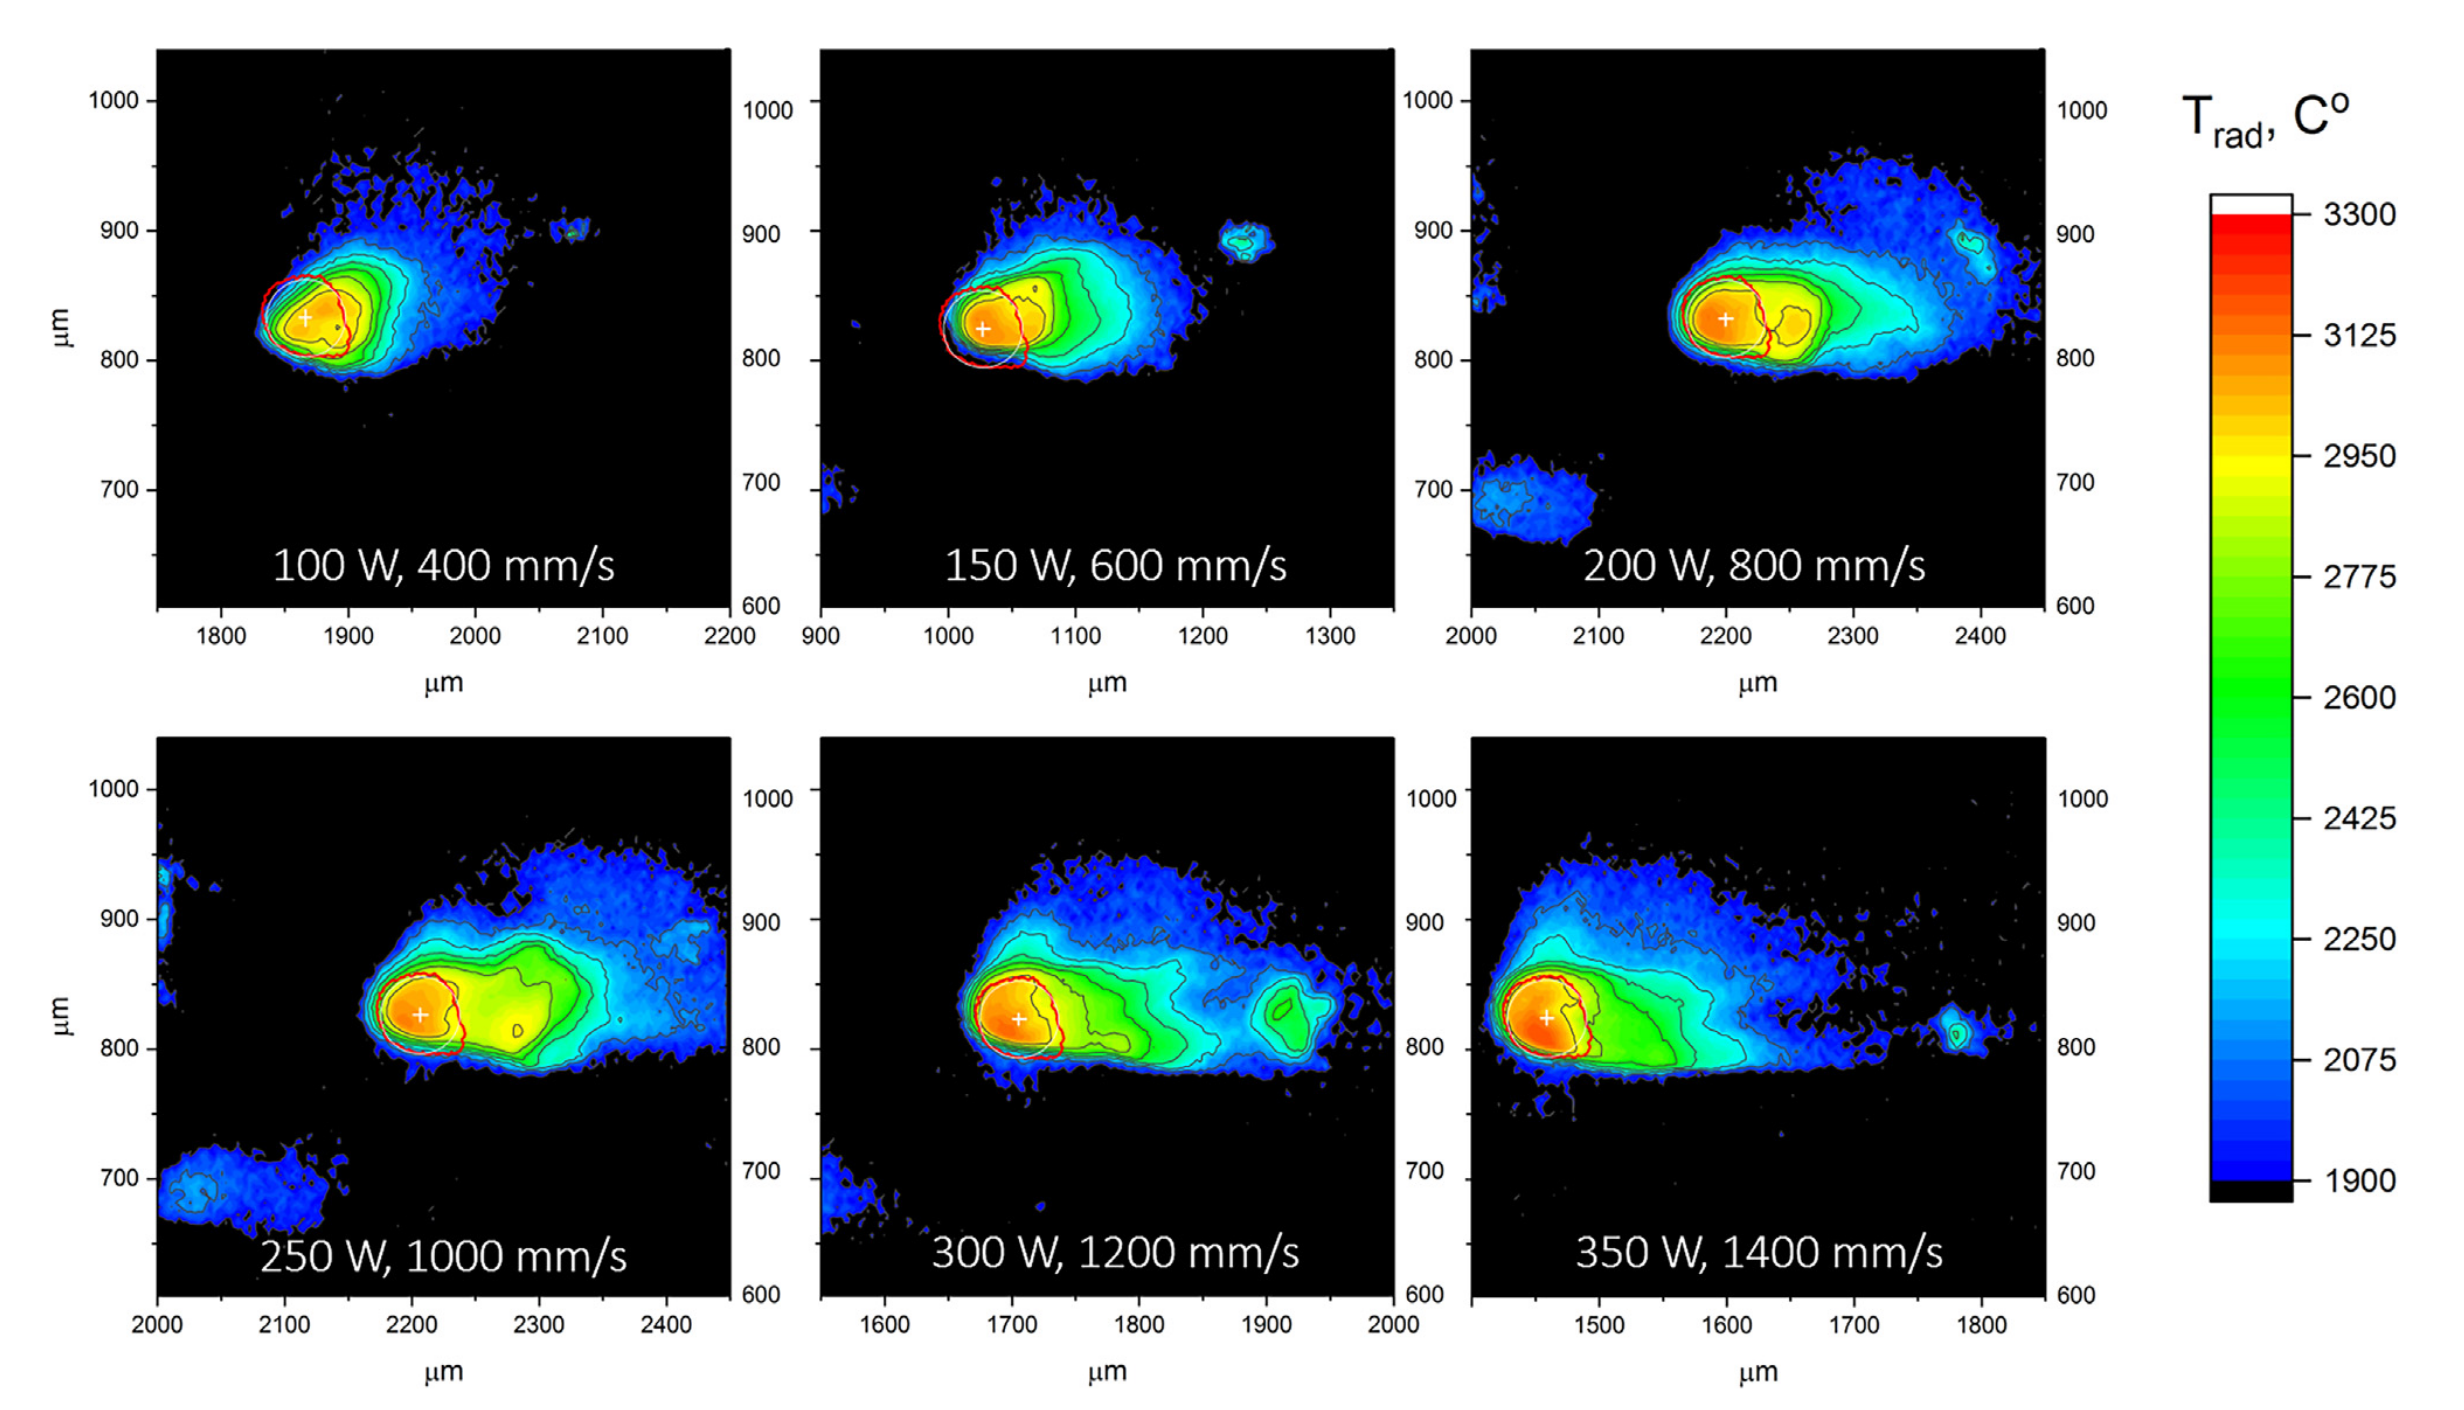
\includegraphics[scale=0.12]{Images/colorini.png}
    }
    \qquad
    \subfloat[\label{fig:spectrograrphy}]{
        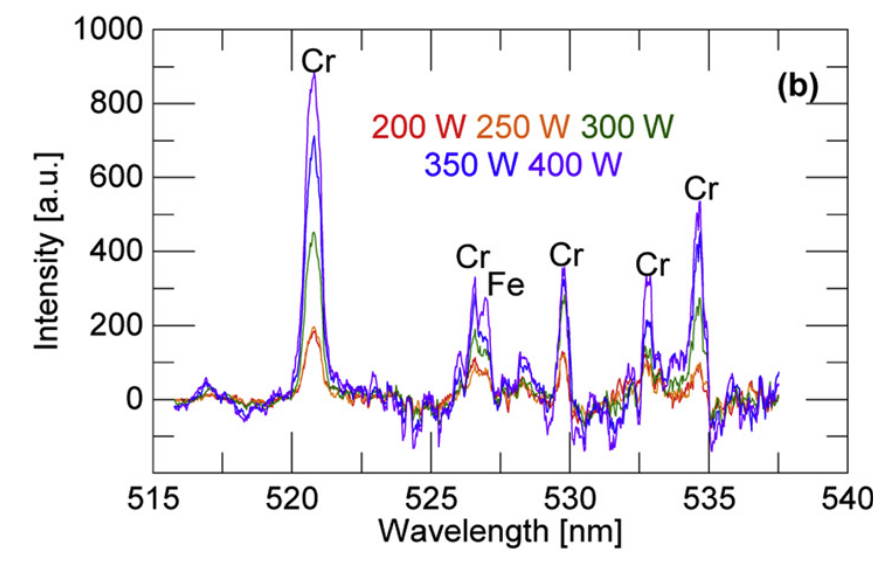
\includegraphics[scale=0.3]{Images/spectrography.png}
    }
    \qquad
    \subfloat[\label{fig:poolthermal}]{
        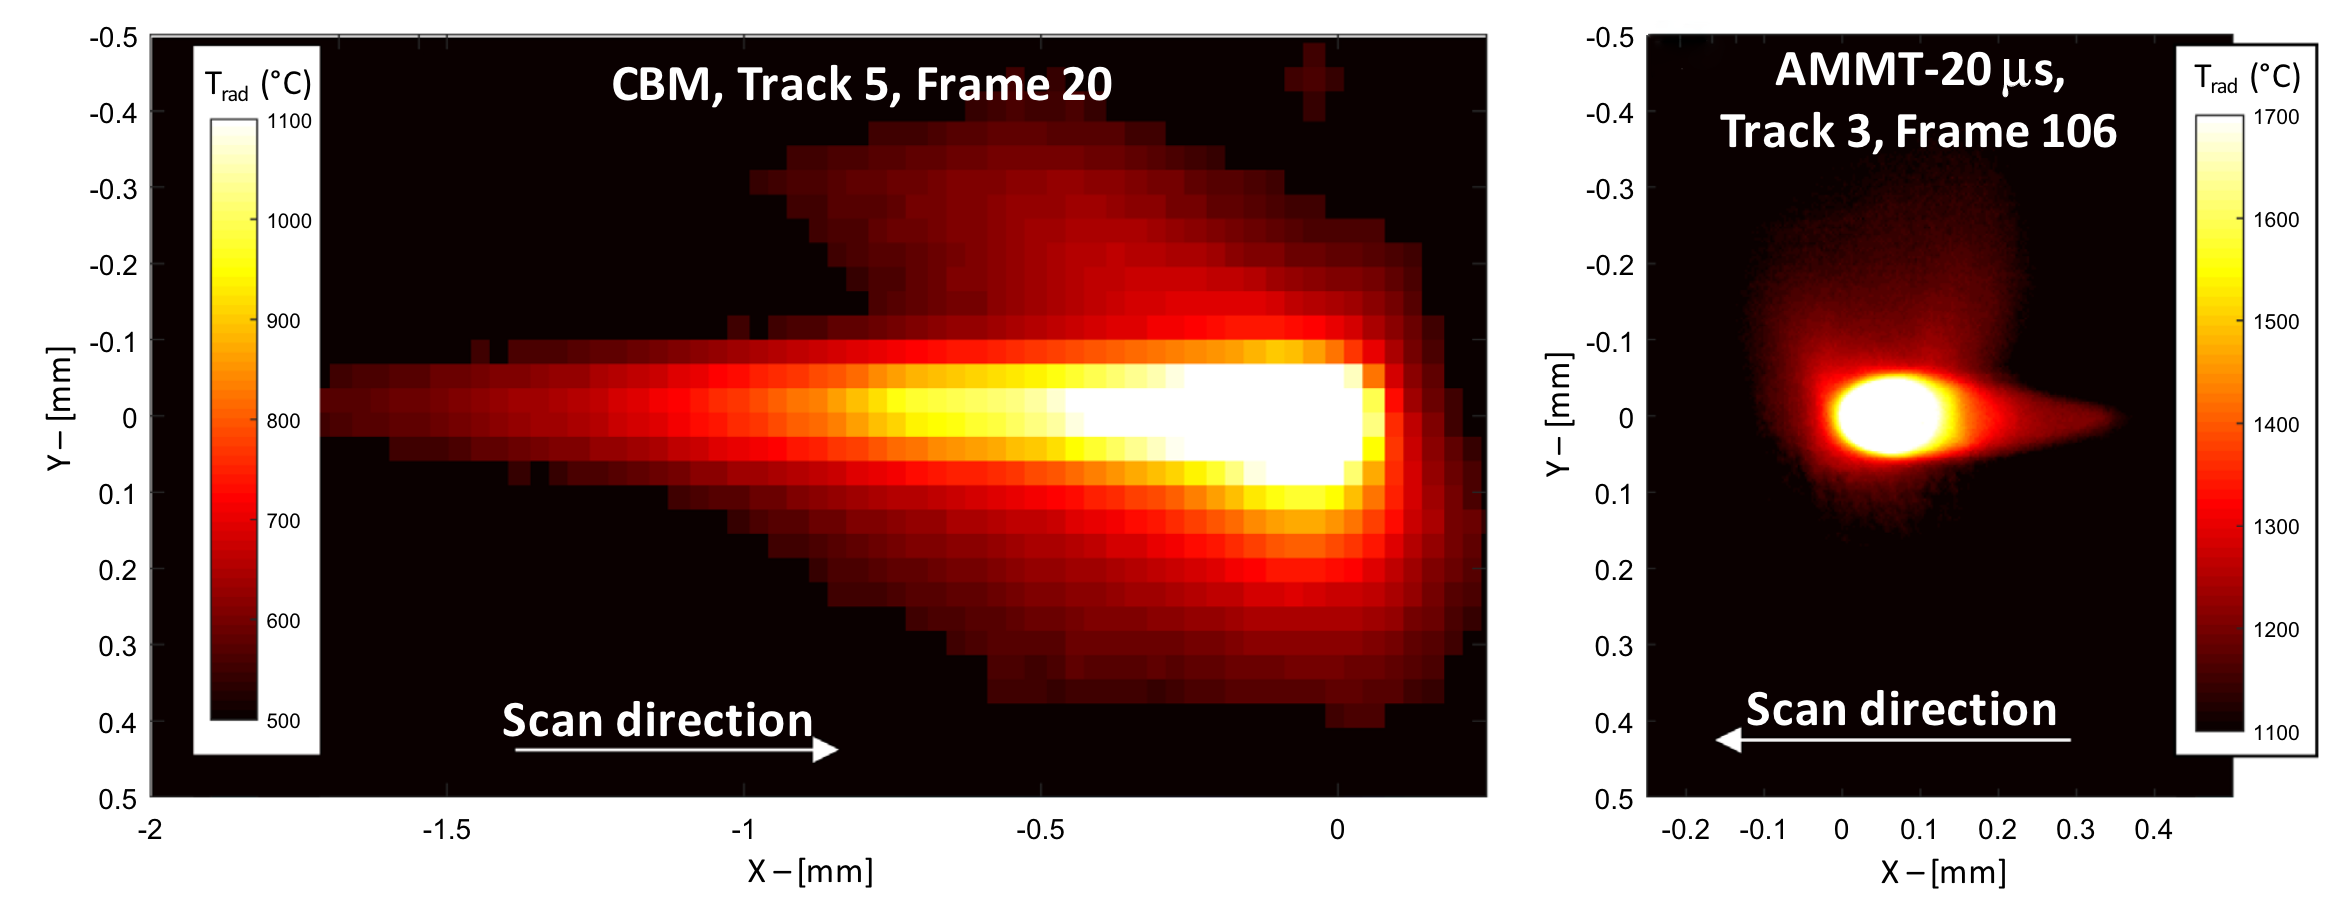
\includegraphics[scale=0.2]{Images/meltpool.png}
    }
    \caption[Level 3 measurement methods.]{Example thermographic video frames aquired using a high speed camera (a) \cite{zhirnov_accurate_2020}, average optical emission spectra of 304L stainless steel (b) \cite{lough_-situ_2020}, and (c) radiance temperature thermal video frames from a thermal camera (left) and high speed camera (right) \cite{lane_measurements_2020}.}
\end{figure}
Another method involves dual-wavelength video imaging, i.e., the acquisition of video sequences at two distinct wavelengths (\SI{700}{\nano\metre} and \SI{950}{\nano\metre}) to enable a temperature estimate via two-colour thermography. This method gets around the problems of guessing the melt pool's brightness by comparing the light levels from the two different wavelengths, thinking they shine consistently at both \cite{williams_situ_2019}.

All the layers discussed so far have one common element: they are used for monitoring the last printed layer, either before, during, or after the melting phase. For \emph{level ~4}, the subject of the monitoring process is under the last layer. Indeed, as the layer is being printed, the material characteristics underneath are also modified due to partial remelting of adjacent layers and heat exchanges within the build volume. Since we cannot use optical devices to monitor what we cannot see, level 4 monitoring relies on other sensors. We can use high-speed, high-energy X-ray imaging systems to gain information about the energy penetration depth and pore formation, or we can use X-ray diffraction measurement to detect any strain and stress formation. Fig. \ref{fig:xray4} shows the result of an X-ray video imaging in L-PBF. Moreover, a new research stream about in-situ X-ray micro-tomography was born recently. In \citeauthor{lhuissier_situ_2020} (2020), during the in-situ microtomography scan, 1500 projections were acquired resulting in a scan time of \SI{45}{s}, gathering a spatial resolution of \SI{3.64}{\micro\metre / pixel}. Another technique regards the in-situ measurements of acoustic emissions (AEs), specifically of structure-borne. This technique also has direct application in industry. Structure-borne AEs are suitable for detecting sudden releases of elastic energy that propagate within the material, allowing us to identify crack formations, detachments of overhang areas from supports, or delamination phenomena. We can also use multiple sensors placed at different locations to triangulate the position of the energy release epicenter. A pioneer in the use of AEs in PBF processes is Rieder. In \citeauthor{rieder_-_2016} (2016), he proposed an ultrasonic monitoring device in L-PBF mounted on the underside of the baseplate focusing on the bottom plate interface echo and the back wall echo patterns as proxies of discontinuities in the specimen.
\begin{figure}
    \centering
    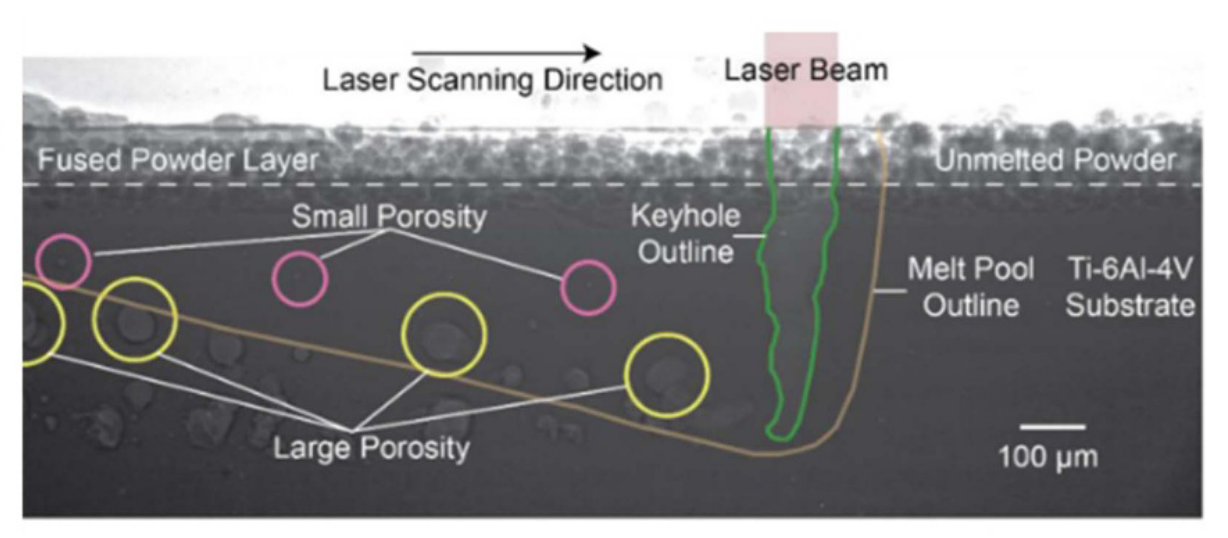
\includegraphics[width=0.65\textwidth]{Images/xray4.png}
    \caption[X-ray video frame.]{Example of an in-situ x-ray video frame with relative defects identified \cite{paulson_correlations_2020}.}
    \label{fig:xray4}
\end{figure}
% <<< End of Sensors for anomalies detection

%%%%%
%%%%%

% Temperature Anomalies and Hot Spots>>>
\section{Temperature Anomalies and Hot Spots}
\label{sec:hotspot}
As discussed in \citeauthor{williams_situ_2019} (2019), almost all major quality characteristics of the final part and its mechanical performance depend on the thermal history of the component. This is because temperatures in PBF systems reach very high values, and the heat might change material mechanical and chemical features. Just the preheating phase can range from \SI{300}{\degreeCelsius} (aluminide) up to \SI{1100}{\degreeCelsius} (titanium aluminide) in EBM \cite{milewski_additive_2017}. Moreover, the surface layer temperature is continually changing throughout the build process. Process parameters do not consider these variations, which can result in increased porosity and differences in local microstructure and mechanical properties, undermining the characteristics of the final part. In \citeauthor{williams_situ_2019} (2019), the authors acquired high-speed videos at \SI{50000}{fps} of the melt-poool region during the printing process of a small cylinder. The images were acquired with a size \numproduct{128x128}\unit{pixels} and a resolution of \SI{20}{\micro\metre / pixel}, using two different wavelengths (\SI{700}{\nano\metre} and \SI{950}{\nano\metre}), so that they could compute temperature using the method described in \citeauthor{hooper_melt_2018} (2018). Each cylinder layer takes approximately \SI{1}{\second} to scan. The cylinder was built with 316L stainless steel using a Renishaw AM250 machine. Fig. \ref{fig:temperatureprofile} shows an example of a temperature profile registered during the printing of the cylinder. The maximum occurs when the laser scans over the measurement point. Due to the sensor's poor temporal and spatial resolution, this cannot be considered the temperature value of the melt pool. However, it is a spatially and temporarily weighted average peak point. Inter-layer cooling time (ILCT) is a significant parameter, and it is defined as the time elapsed between two consecutive peaks, i.e., between two consecutive scan phases. The minimum peaks are recorded twice per layer, as the printer has only one powder tank. The first minimum occurs when the blade returns to the reservoir to draw new powder, and the second occurs once the new powder layer is deposited. As proof that the layer temperatures are constantly changing, we can see an increase in pixel intensity after the second minimum. This is because the newly spread powder surface has a higher emissivity than the consolidated layer below, producing a higher IR emission intensity for a given temperature.
\begin{figure}
    \centering
    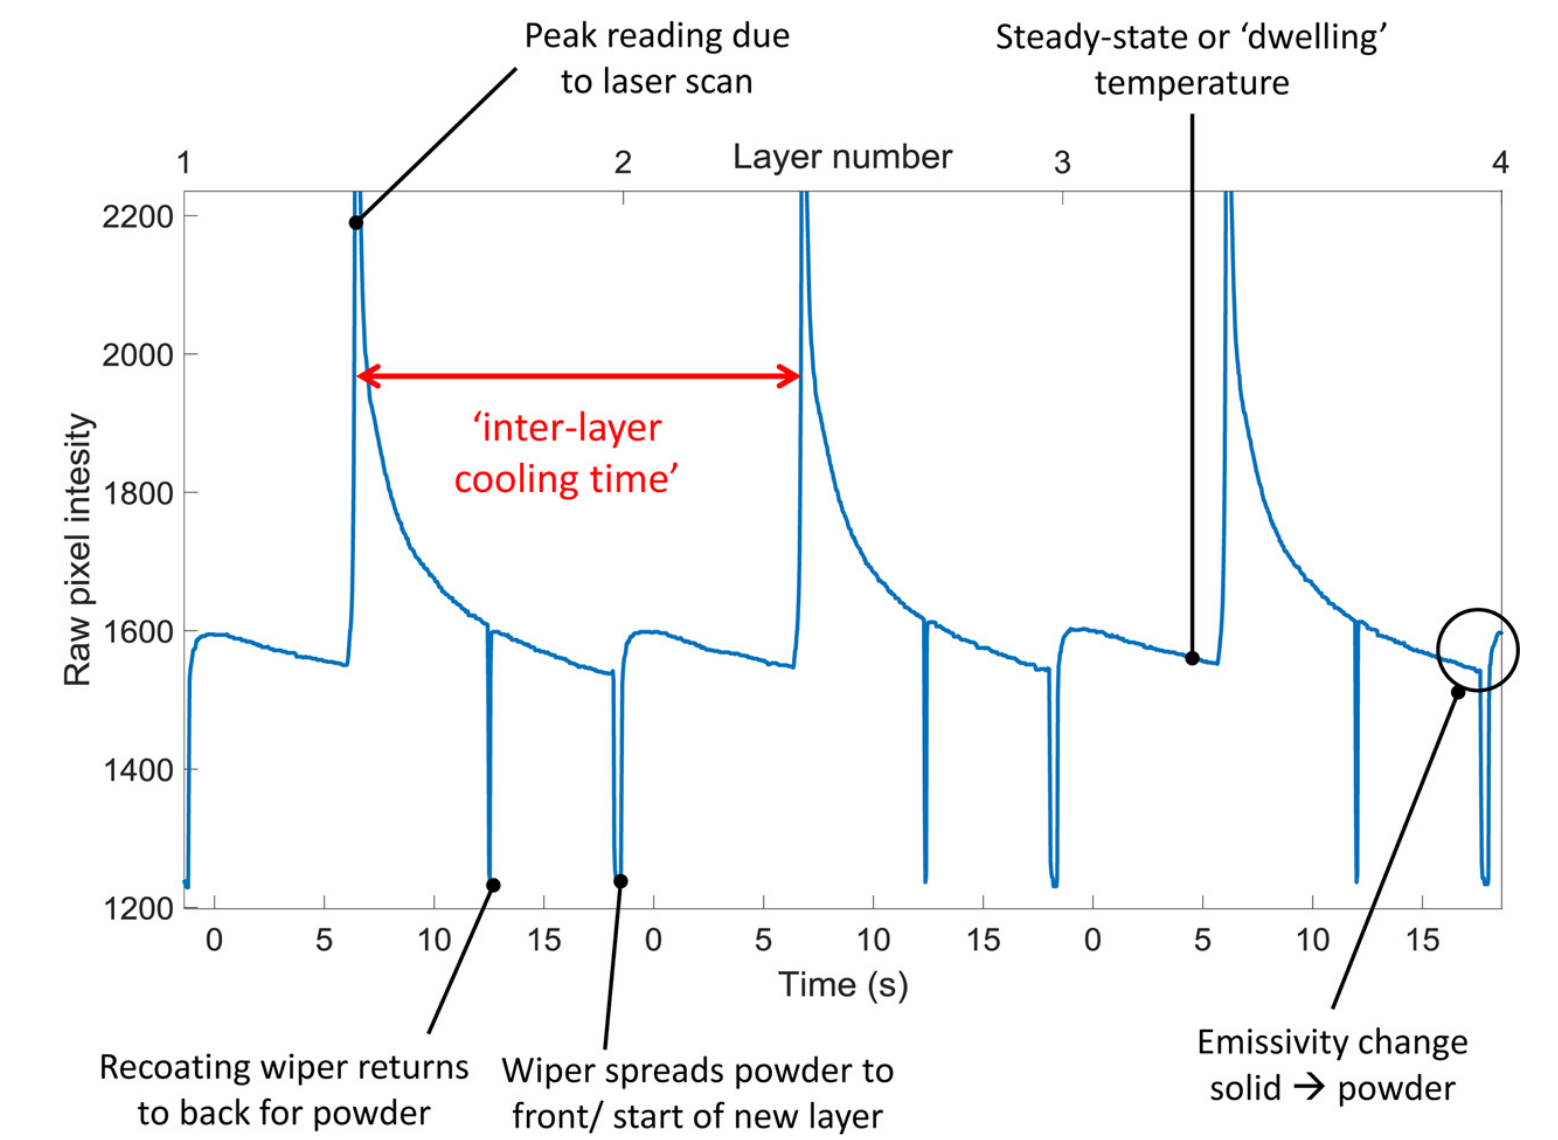
\includegraphics[width=0.6\textwidth]{Images/temperature profile.png}
    \caption[Temperature profile.]{Annotated plot of the thermal cycle experienced at a location on the part surface during three layers of a build \cite{williams_situ_2019}.}
    \label{fig:temperatureprofile}
\end{figure}
The authors proposed the following experiment to test the impact of ILCT and temperature peaks on the final piece. Eight short cylinders, each with a diameter of 8 mm and a height of 20 mm, were constructed alongside a taller cylinder measuring 60 mm in height. During the initial 20 mm of the building process, while all the cylinders were being scanned, the ILCT was approximately 20 seconds. In the middle segment, when only the tall cylinder was undergoing scanning, the ILCT was approximately 11 seconds. At a height of 40 mm, the author introduced eight short cylinders of identical dimensions, using a 5 W laser power to extend the scanning duration, resulting in an ILCT of approximately 20 seconds. Due to the significantly reduced laser power (the default laser power on Reinshaw AM250 is 200 watts), no melting occurred, and only a feeble sintering effect was obtained. Fig. \ref{fig:williamporosities} shows microscope images of the etched microstructure with a 20$\times$ objective lens in the lower, middle, and upper sections.
\begin{figure}
    \centering
    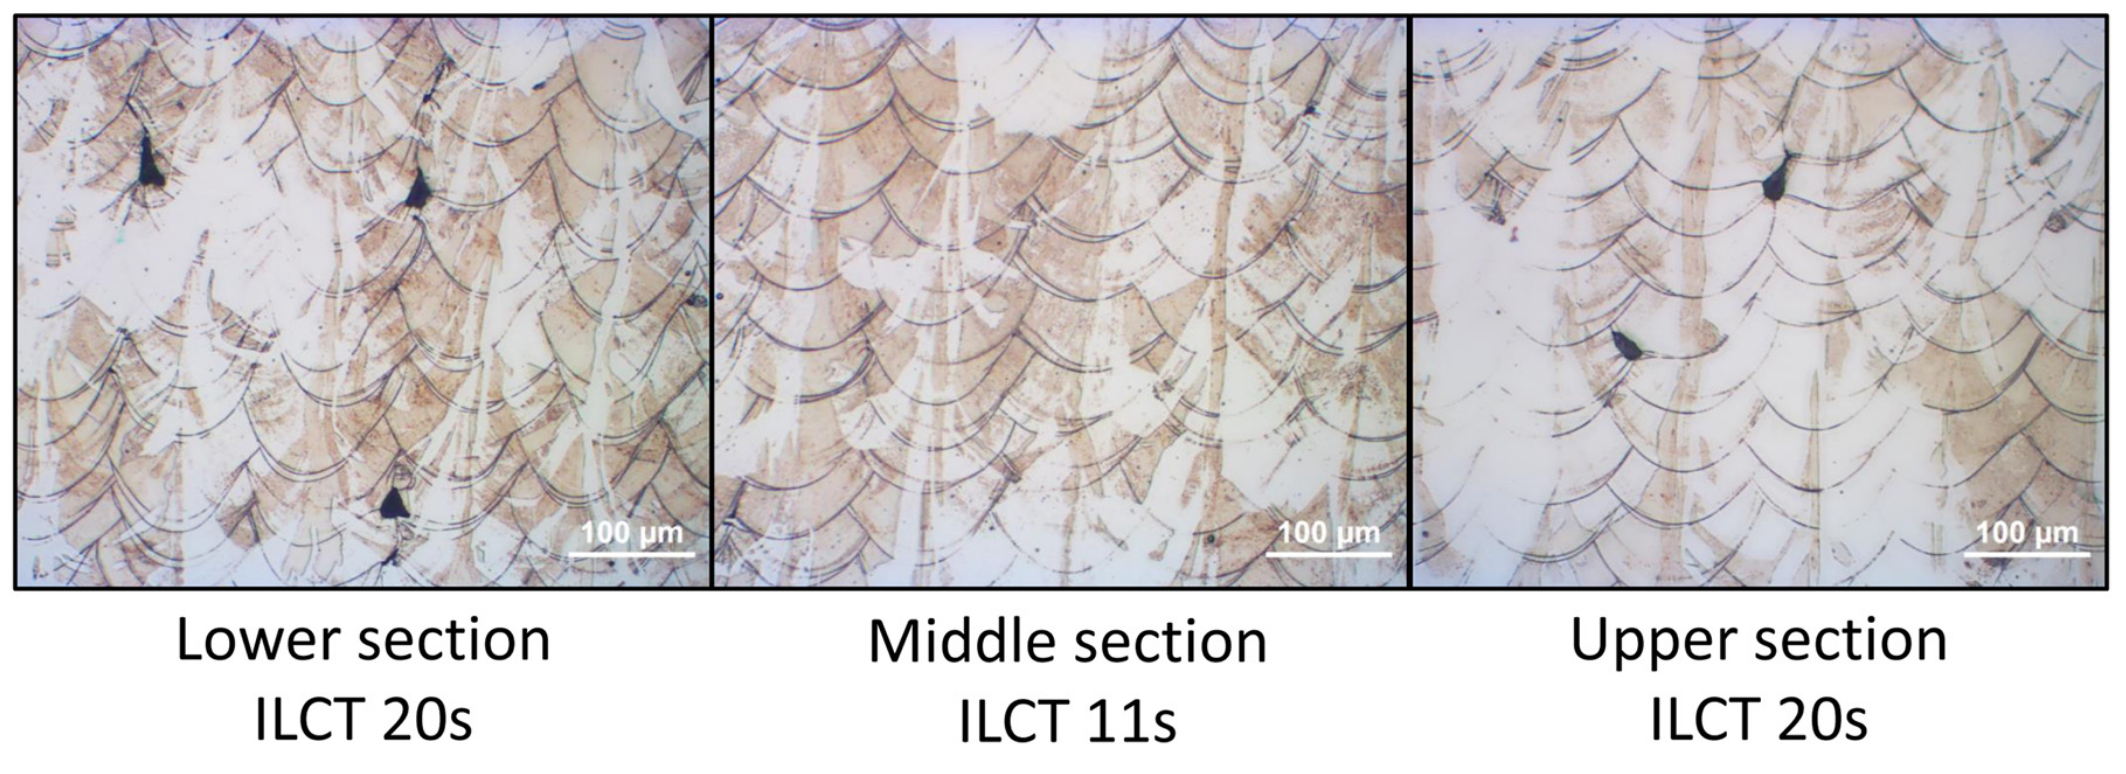
\includegraphics[width=0.8\textwidth]{Images/differntisezioni.png}
    \caption[Microstructure of reference cylinder.]{Etched OM images of the microstructure taken at the center height of each of the three regions: lower (10 mm), middle (30 mm), and upper (50 mm). The percentage porosity of each region is annotated above (not a measure of porosity in the image, but the region as a whole) \cite{williams_situ_2019}.}
    \label{fig:williamporosities}
\end{figure}
ILCT and maximum temperature affect the printed cylinder's porosity and microstructure. We can see from Fig. \ref{fig:williamporosities} that the middle section has much lower porosity than the other two sections. Pores can be explained by areas of lack of fusion (LOF), areas where the powder has not appropriately melted. Moreover, the lower section is characterized by many fine grains with few coarse grains. In contrast, the middle section exhibits a more significant fraction of coarse grains. Finally, the grain structure of the upper section appears very similar to the middle section. Average grain sizes were found to be of \num{20.4}, \num{23.9}, and \num{23.7} \unit{\micro\metre} for the lower, middle, and upper sections, respectively. Finally, the authors used the Vickers hardness test to measure the mechanical properties of the printed part. The test results can be seen in table \ref{table:hard}. Although these differences are small, the values suggest longer ILCT results in higher hardness values. Confidence intervals suggest that the rise in hardness between the lower and middle sections is likely accurate. Nevertheless, distinctions in hardness between the central and upper segments might not be accurate, and the segments could share the same actual mean value.
\begin{table}
\footnotesize
    \centering 
    \begin{tabular}{|l l l l|}
    \hline
    %\rowcolor{bluepoli!40} % comment this line to remove the color
    Section & \makecell{Mean hardness \\(HV10)} & \makecell{95\% upper \\confidence bound} & \makecell{95\% lower \\ confidence bound} \T\B \\
    \hline \hline
    Lower & 217.8 & 219.0 & 216.7  \T\B \\ 
    Middle & 213.3 & 214.5 & 212.1  \T\B \\ 
    Upper & 214.3 & 215.7 & 223.0  \T\B \\ 
    
    \hline
    \end{tabular}
    \\[10pt]
    \caption{Mean hardness values and 95\% upper and lower confidence bounds for values measured in each of the three sections \cite{williams_situ_2019}.}
    \label{table:hard}
\end{table}
The residual heat is another phenomenon involving the anomalous behavior of temperature profiles. Indeed, after powder recoating, the new, not yet solidified layer is affected by the residual heat of the previous layer. This heat transfer between layers is essential for the printing process because it allows, through the partial melting of the new layer, a better adhesion between the layers and a higher resolution of the finished piece. However, this phenomenon also affects material porosity or microstructures. Fig. \ref{fig:residualheat} shows an example of residual heat phenomenon, and Fig. \ref{fig:hstermo} shows an example of an OOC residual heat.
\begin{figure}
    \centering
    \subfloat[\label{fig:residualheat}]{
        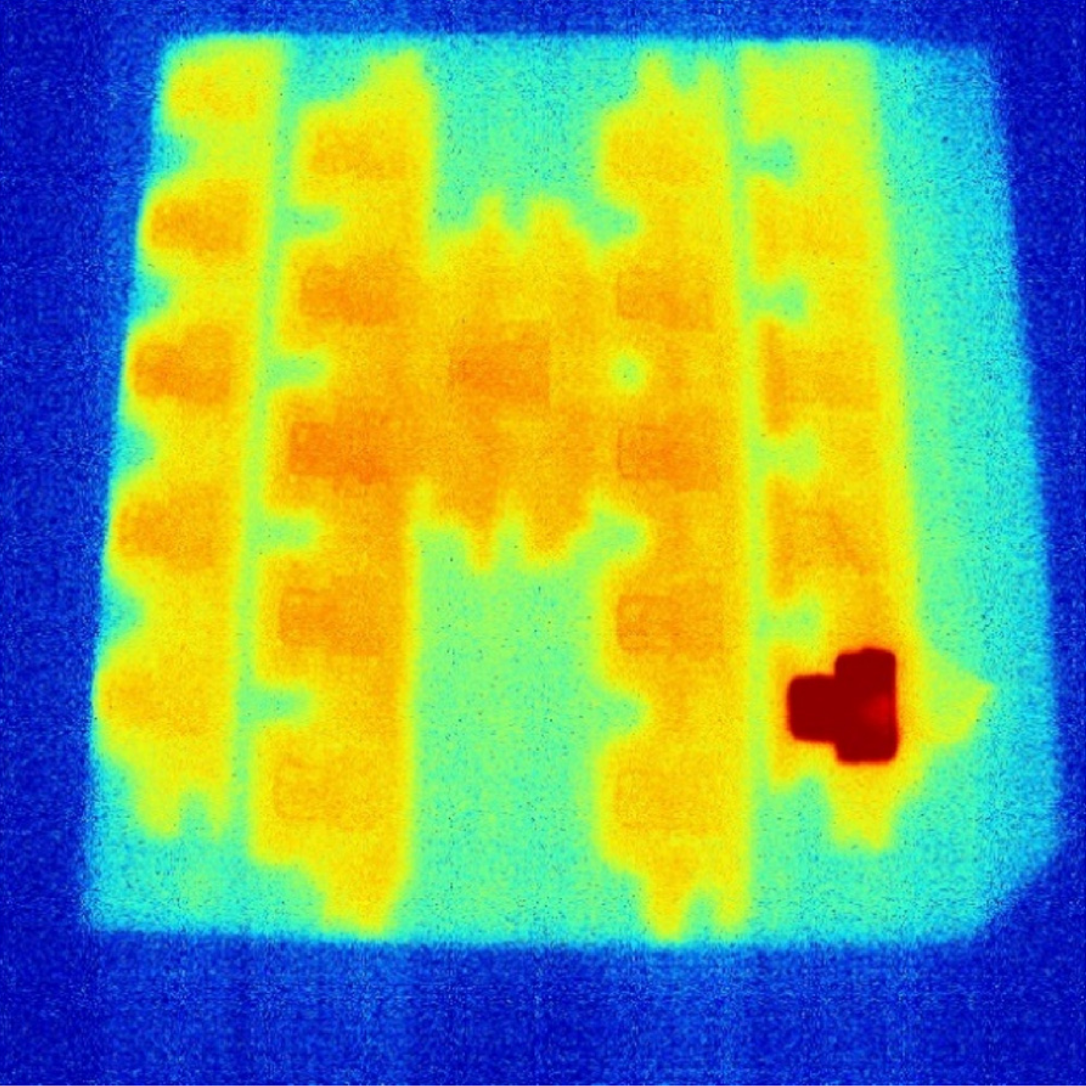
\includegraphics[scale=0.20]{Images/residualHS.png}
    }
    \\
    \subfloat[\label{fig:hstermo}]{
        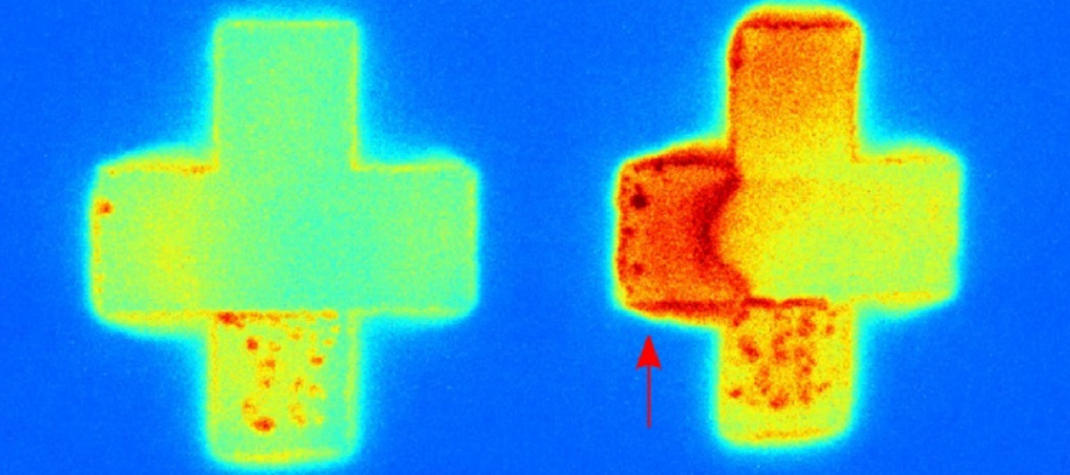
\includegraphics[scale=0.25]{Images/HStermo.png}
    }
    \quad
    \subfloat[\label{fig:hsrisultati}]{
        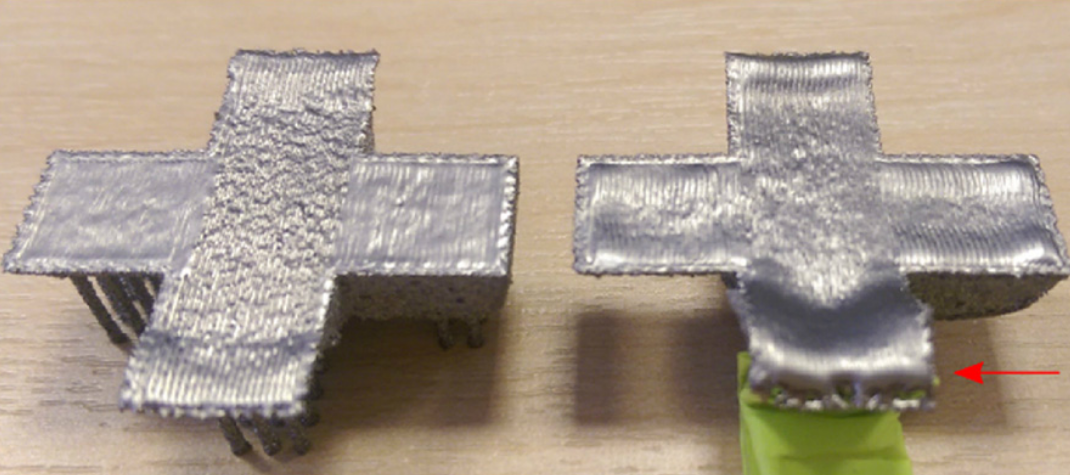
\includegraphics[scale=0.25]{Images/risultatiHS.png}
    }
    \caption[Residual heat.]{Examples of residual heat phenomenon. The phenomenon of residual heat (a), zoom on the lower left side showing an abnormal residual heat situation (b), and the results on the finished part (c). The red arrow indicates the most critical part in both photos \cite{boone_thermal_2018}.}
\end{figure}
This defect characterized by anomalous area temperature profiles is known as a hot spot (HS). The primary cause of these defects is the laser beam repeatedly scanning of thermally insulated regions. These areas are predominantly surrounded by powder and lack any support structure to ensure the proper cooling down phase and overhanging walls and sharp edges. Thus, the localized printing parameters, such as the scan strategy and the direction of heat extraction (depending on geometry), can explain the observed phenomena of hot spot and dross shifting. Furthermore, as demonstrated in \citeauthor{moshiri_performance_2023} (2023), geometric features can also lead to the formation of HS, especially for parts suspended without supports to aid the cooling process. The localized overheating of the powder bed leads to the following defects \cite{bugatti_towards_2022}:
\begin{itemize}
    \item \textbf{High surface roughness:} overheated areas can lead to melting unwanted areas of powder, and partially melted powder particles attach to the surface. This will result in small melted powder on the surface of the final object, thus increasing its roughness;
    \item \textbf{Change in material microstructure:} normal melting zones are characterized by a high cooling rate that leads to finer grain formation, while overheating regions tend to develop a coarser microstructure due to the slower cooling transient;
    \item \textbf{Porosity formation:} if the region is already hot, new laser scans may lead to material vaporization. Hence, unstable keyhole formation is often correlated with porosity defects.
\end{itemize} An example of defects generated by hot-spot can be seen in Fig. \ref{fig:cane}.
\begin{figure}
    \centering
    \subfloat[\label{fig:dio}]{
        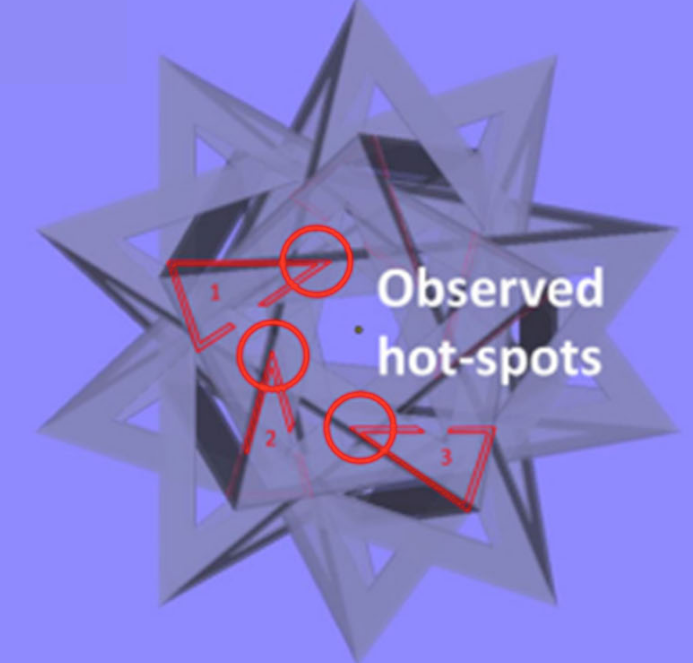
\includegraphics[scale=0.45]{Images/modehs.png}
    }
    \qquad
    \subfloat[\label{fig:cane}]{
        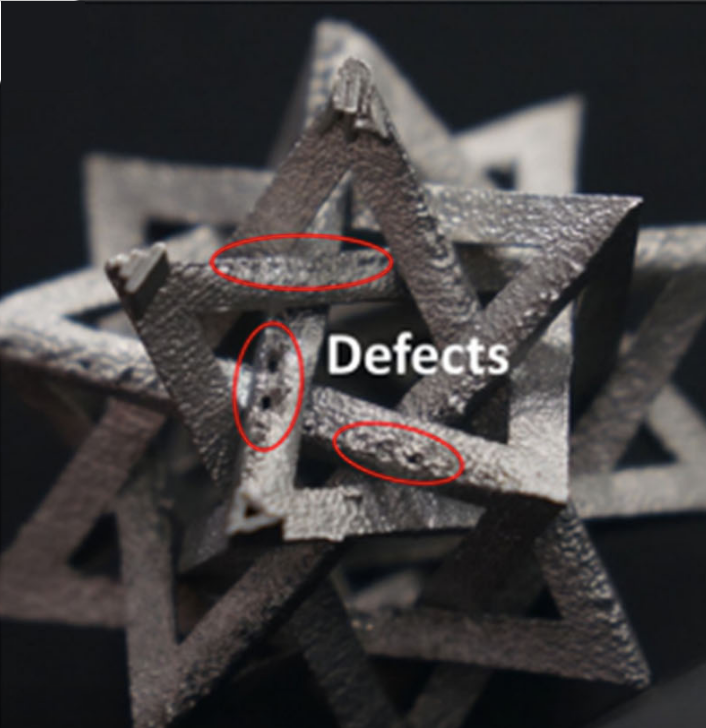
\includegraphics[scale=0.4]{Images/printedhs.png}
    }
    \caption[Examples of hot spot defects.]{Examples of a complex shape CAD model with the position of the observed hot spot (a) and relative observed defects in printed part (b) \cite{grasso_-process_2017}.}
    \label{fig:complexhs}
\end{figure}
A hot-spot region remains hot (bright) for longer and has a slower cooling drift than standard areas. Thus, the thermal profile will have a higher maximum than the thermal profiles of the areas in control and a different ILCT from the expected one. Referring to Fig. \ref{fig:temperatureprofile}, the slope of the thermal profile after the maximum peak will be lower. In mathematical terms, the velocity, hence the first derivative of the heat profile with respect to time, will be lower. Therefore, a conventional camera that detects pixel intensity with sufficient temporal resolution is more than sufficient to identify these anomalies, as in \citeauthor{grasso_-situ_2021} (2020). \citeauthor{boone_thermal_2018} (2018) employed an optical sensor for video-imaging in the NIR range. The main advantage is that it filters out specific wavelengths and reduces the dynamic range of the video compared to traditional optical video imaging methods.
% <<< End of Temperature Anomalies and Hot Spots